\documentclass[12pt,a4paper]{report}
\linespread{1.2}

\usepackage{amsmath,amssymb,amsfonts}
\usepackage{algorithmic}
\usepackage{graphicx}
\usepackage{xcolor}
\usepackage{multirow}
\usepackage{longtable}
\usepackage{float}
\usepackage{listings}
\usepackage{listings-golang}
\lstset{ % add your own preferences
    frame=single,
    basicstyle=\linespread{0.9}\footnotesize\ttfamily,
    keywordstyle=\color{red},
    numbers=left,
    numbersep=5pt,
    showstringspaces=false, 
    stringstyle=\color{blue},
    tabsize=4,
    language=Golang % this is it !
}
% \lstdefinelanguage{yaml}{
%   keywords={true,false,null,y,n},
%   keywordstyle=\color{darkgray}\bfseries,
%   ndkeywords={},
%   ndkeywordstyle=\color{black}\bfseries,
%   identifierstyle=\color{black},
%   sensitive=false,
%   %moredelim=[l]{}{:},
%   comment=[l]{#},
%   morecomment=[s]{/*}{*/},
%   commentstyle=\color{purple}\ttfamily,
%   stringstyle=\color{blue}\ttfamily,
%   %morestring=[l]{-}{},
%   morestring=[b]',
%   morestring=[b]"
% }
\usepackage[font={small,it}]{caption}
\usepackage{subcaption}
\usepackage[english,ngerman]{babel}
\usepackage[backend=biber,
            sorting=none,   % Keine Sortierung
            doi=true,       % DOI anzeigen
            isbn=true,      % ISBN nicht anzeigen
            url=true,       % URLs anzeigen
            maxnames=6,     % Ab 6 Autoren et al. verwenden
            minnames=1,     % und nur den ersten Autor angeben
            style=numeric-comp,]{biblatex}
\addbibresource{literatur.bib}
\usepackage[colorlinks=true,
            urlcolor=black,
            linkcolor=black,
            filecolor=black,
            citecolor=black,]{hyperref}
\usepackage{fancyhdr}
% \pagestyle{fancy}
% \fancyhf{}
% \rhead{\thechapter}
% \cfoot{\thepage}

\def\BibTeX{{\rm B\kern-.05em{\sc i\kern-.025em b}\kern-.08em
    T\kern-.1667em\lower.7ex\hbox{E}\kern-.125emX}}

\begin{document}

\begin{titlepage}
    \noindent
\includegraphics[width=7cm]{img/hs_logo.png}
    \begin{center}
        \sffamily
        \Large
        \textbf{Ein Proxy zur Erzeugung, Aufzeichnung und Wiedergabe von Netzwerk-Unterbrechungen in einer Testumgebung für verteilte Systeme}

        \vspace{1cm}

        \large
        \begin{Large}Jonathan Arns\end{Large}

        \vspace{1.5cm}
                
        
        \textb{Bachelor-Thesis}\\
        \begin{small}zur Erlangung des akademischen Grades Bachelor of Science (B.Sc.)\end{small}\\
        \textb{Studiengang Unternehmens- und Wirtschaftsinformatik}

        \vspace{1cm}
                
        Fakultät für Informatik\\
        \begin{Large}Hochschule Mannheim\end{Large}\\
        
        \vspace{1cm}
        15.11.2021

        \vfill

        Betreuer\\
        Prof. Dr. Oliver Hummel, Hochschule Mannheim\\
        Prof. Dr. Thomas Smits, Hochschule Mannheim\\
   \end{center}
\end{titlepage}

\tableofcontents
\setlength{\parindent}{0em}
\setlength{\parskip}{0.6em}

%%%%%%%%%%%%%%%%%%%%%%%%%%%%%%%%% Document beginning %%%%%%%%%%%%%%%%%%%%%%%%%%%%%%%%%%%%%%

\begin{abstract}
	Das ist das abstract, das werde ich wohl am Ende schreiben.
	% Problem
	% Idea
	% Benefit
	% Approach
\end{abstract}


\chapter{Einleitung}
% Background
% Verteilte Systeme sind heute überall. Das ist eine vergleichsweise neue Entwicklung.
Verteilte Systeme sind heute kritisch für viele Anwendungsfälle in der Informatik von Social Media über Streaming-Anbieter bis hin
zu Machine-Learning.

% Problem
Verteile Systeme bringen Herausforderungen und potentielle Fehler mit sich, die in alleinstehenden Prozessen meist nicht
auftreten. Eine davon ist, dass in verteilten Systemen oft einzelne Komponenten des Systems fehlschlagen, anstelle des ganzen
Systems. Um die Verfügbarkeit und Korrektheit von Systemen zu garantieren, ist es wichtig, verteilte Systeme zu entwickeln, die
sich von diesen Fehlern selbstständig erholen und weiter funktionieren können. \cite{distributed_systems_book}

Eine häufige Annahme, die problematisch ist, ist dass das Netzwerk, welches zur Kommunikation verwendet wird,
fehlerfrei ist \cite{brief_introduction_to_distributed_systems, the_network_is_reliable}. In der Realität sorgen
Netzwerk-Unterbrechungen und andere Fehler dafür, dass die Kommunikation innerhalb verteilter Systeme grundsätzlich unzuverlässig
ist \cite{distributed_systems_book, distributed_systems_concepts_and_design}. Verteilte Systeme müssen also auch in der Gegenwart
von Netzwerk-Unterbrechungen die Integrität des jeweiligen System und seiner Daten garantieren. Obwohl das Problem an sich bereits
intensiv erforscht ist, führen Netzwerk-Unterbrechungen weiterhin zu schwerwiegenden Fehlern in vielen wichtigen
Produktionssystemen \cite{analysis_of_network_partition_failures}. Dazu trägt unter Anderem ein Mangel an Test- und
Debugging-Tools für diesen Zweck bei \cite{failify_paper,simple_testing_can_prevent}, der eine Folge der rasanten Entwicklung
moderner Cloud-Infrastruktur ist \cite{why_does_cloud_stop_computing}. Zwar gibt es bereits Tools, die effektiv darin sind, neue
Bugs zu finden, diese sind aber nicht in der Lage, gefundene Bugs deterministisch zu reproduzieren \cite{failify_paper}. Das ist
sowohl für das Erstellen von Regressionstests, als auch beim Debugging ein Problem.

% Forschungsfrage: Können durch Netzwerk-Unterbrechungen ausgelöste Bugs in einer Testumgebung für verteilte Systeme erzeugt,
% aufgezeichnet und deterministisch wiedergegeben werden? - unabhängig von technologie des systems

% Idea
Record-and-Replay ist ein Debugging-Ansatz, welcher es ermöglicht, selbst komplexe Bugs deterministisch zu reproduzieren.
Existierende Replay-Debugger für verteilte Systeme sind allerdings wenig ausgereift und beschränken sich auf Systeme in bestimmten
Programmiersprachen \cite{distributed_replay_debugging_1997,distributed_replay_debugging_2006}. Diese Arbeit stellt ein Konzept
und einen Prototyp für einen auf Netzwerk-Unterbrechungen spezialisieren Replay-Debugger vor, welcher
Programmiersprachen-agnostisch Bugs in verteilten Systemen reproduzieren kann.

% Benefit

% Approach
Der verfolge Ansatz für ein solches Tool ist eine Testumgebung, welche einen Proxy verwendet, um Netzwerk-Unterbrechungen zu
erzeugen. Dieser Proxy zeichnet zusätzlich den gesamten Netzwerk-Verkehr des Systems inklusive Metadaten auf, um die erzeugten
Netzwerk-Unterbrechungen später in einem Replay gleich wiedergeben zu können. Eine graphische Oberfläche stellt den
Netzwerk-Verkehr und die Log-Ausgaben des System under Test (SUT) gemeinsam chronologisch sortiert dar, um dem Nutzer einen bei
der Identifikation von Bugs zu helfen.

% Overview
Zu Anfang der Arbeit werden zunächst die technischen Grundlagen über verteilte Systeme, Netzwerk-Unterbrechungen und relevante
Technologien erläutert. Im Anschluss folgt eine Darstellung des aktuellen Stands der Technik, sowie offener Forschungsfragen und
noch fehlender Entwicklungen im Forschungsgebiet. Kapitel \ref{chap:system} knüpft daran an, indem im Detail die verfolgte Idee
und der daraus entwickelte Prototyp beschrieben wird.

Für die empirische Evaluation des Prototypen werden erst alle entworfenen Experimente berschrieben, bevor in Kapitel
\ref{chap:results} die Ergebnisse zusammengefasst werden. Im Anschluss werden alle Ergebnisse und deren Einschränkungen
diskutiert. Basierend auf den Gesamtergebnissen der Arbeit werden Empfehlungen sowohl für eine Weiterentwicklung den Konzepts
gegeben.
% als auch für weitere Forschung im Allgemeinen gegeben.

\chapter{Grundlagen}

\section{Verteilte Systeme}
% kontext der Arbeit sind verteilte systeme, die heute sich auf virtualisierung, dev ops, cloud native verlassen
Gunawi et. al. \cite{distributed_systems_concepts_and_design} definieren eine verteiltes System als ein System, in dem Hardware-
oder Software-Komponenten, die auf oder an vernetzten Rechnern laufen, untereinander kommunizieren und ihre Aktionen
ausschließlich mittels Nachrichten über das Netzwerk koordinieren. Van Steen et. al.
\cite{brief_introduction_to_distributed_systems} fügen dieser Definition hinzu, dass die jeweils autonomen Komponenten gemeinsam
einem Nutzer des Systems gegenüber wie ein einziges System erscheinen. Ein Nutzer kann dabei sowohl ein Mensch, als auch eine
Applikation sein.

\cite{cloud_virtualization}

% We define a distributed system as one in which hardware or software components
% located at networked computers communicate and coordinate their actions only by
% passing messages. This simple definition covers the entire range of systems in which
% networked computers can usefully be deployed. \cite{distributed_systems_concepts_and_design}
\subsection{Verteilter Consens}
\cite{raft_original_paper}

\section{Netzwerk-Unterbrechungen}
Eine Netzwerk-Unterbrechung ein einem verteilten System ist eine Situation, in der ein Teil des Netzwerks ausfällt, sodass Teile
des Systems, die eigentlich miteinander kommunizieren können sollten, sich nicht mehr erreichen können. Netzwerk-Unterbrechungen
können zu fatalen Folgen, wie dem Verlust oder der Korruption von Daten, führen. Sie können außerdem auf ganz unterschiedlichen
Größenordnungen auftreten, sowohl zwischen geographisch unterschiedlich gelegenen Data-Centern, als auch zwischen Rechnern im
gleichen Data-Center. \cite{analysis_of_network_partition_failures}

Zwar gibt es keine zuverlässigen Zahlen dazu, wie oft Netzwerk-Unterbrechungen auftreten, auch deshalb, weil Netzwerk nicht gleich
Netzwerk ist und die Unterschiede auch im Bezug auf die Häufigkeit und Dauer von Netzwerk-Unterbrechungen sehr groß sind. Aus
anekdotischen Berichten und internen Studien großer Unternehmen lässt sich trotzdem schließen, dass Netzwerk-Unterbrechungen nicht
nur ein akademisches Problem sind, sondern auch in der Realität auftreten und Schaden anrichten. Aus diesem Grund ist es wichtig,
verteilte Systeme so zu entwerfen, dass sie mit Netzwerk-Unterbrechungen umgehen können. \cite{the_network_is_reliable}

\subsection{Arten von Netzwerk-Unterbrechungen}
Netzwerk-Unterbrechungen lassen sich in drei Kategorien einteilen. Vollständige Netzwerk-Unterbrechungen wie in Abbildung
\ref{fig:full_partition} trennen ein verteiltes System in zwei komplett alleinstehende Teile. Sie sind die häufigste Art von
Netzwerk-Unterbrechung und können sowohl zwischen verschiedenen Data-Centern, als auch zwischen Teilen eines Systems im gleichen
Data-Center auftreten. Teilweise Netzwerk-Unterbrechungen wie in Abbildung \ref{fig:partial_partition} trennen einen Teil des
Systems von einem Anderen, während ein dritter Teil des Systems weiterhin beide anderen Teile erreichen kann. Sie entstehen, indem
zwei Data-Center voneinander getrennt werden, die beiden weiterhin von einem dritten Data-Center erreichbar sind. Einseitige
Netzwerk-Unterbrechungen wie in \ref{fig:simplex_partition} lassen Nachrichten nur in eine Richtung fließen. Diese Art von
Netzwerk-Unterbrechung tritt selten auf und wird ausgelöst durch fehlerhafte Konfigurationen oder Hardware-Fehler.
\cite{analysis_of_network_partition_failures}

\begin{figure}[H]
	\centering
	\begin{subfigure}{.495\textwidth}
		\centering
		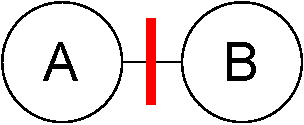
\includegraphics[width=.8\linewidth]{img/ditm-Partitions-full.pdf}
		\caption{Vollständige Netzwerk-Unterbrechung: Das System ist in zwei alleinstehende Teile getrennt.
			\cite{analysis_of_network_partition_failures}}
		\label{fig:full_partition}
	\end{subfigure}
	\begin{subfigure}{.495\textwidth}
		\centering
		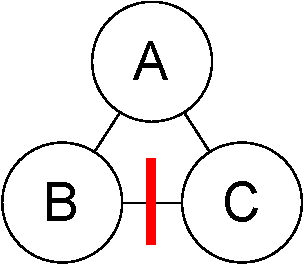
\includegraphics[width=.85\linewidth]{img/ditm-Partitions-partial.pdf}
		\caption{Teilweise Netzwerk-Unterbrechung: Teile des Systems sind voneinander getrennt, aber nicht alle Knoten des Systems
			sind betroffen. \cite{analysis_of_network_partition_failures}}
		\label{fig:partial_partition}
	\end{subfigure}
	\begin{subfigure}{.495\textwidth}
		\centering
		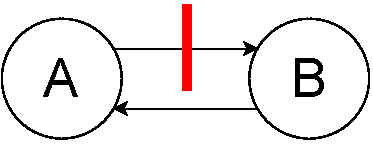
\includegraphics[width=\linewidth]{img/ditm-Partitions-simplex.pdf}
		\caption{Einseitige Netzwerk-Unterbrechung: Nachrichten können nur in eine Richtung fließen.
			\cite{analysis_of_network_partition_failures}}
		\label{fig:simplex_partition}
	\end{subfigure}
	\caption{Arten von Netzwerk-Unterbrechungen}
	\label{fig:partition_types}
\end{figure}

\subsection{Partitionstoleranz und CAP}
\cite{cap_brewer}
\cite{perspectives_on_cap}

\subsection{Linearisierbarkeit}
\cite{linearizability_paper}



\chapter{Stand der Technik}
Im Umgang mit Fehlern in verteilten Systemen werden eine Reihe verschiedener Ansätze mit unterschiedlichen Zielen verfolgt.
Failure Testing und Chaos Engineering sind zwei ähnliche Methoden, die sich darauf verlassen, Fehler mit Hilfe von Tests zu
finden, mit dem Unterschied, dass Failure Testing in einer Testumgebung und Chaos Engineering in der Produktions-Umgebung
eingesetzt werden. Daneben gibt es Log-Analyse und Tracing-Systeme, die vor allem dazu dienen, aufgetretene Fehler
nachzuvollziehen. Zu diesem Zweck gibt es ebenfalls eine Handvoll weiterer, oft experimenteller Debugging-Tools. Diese reichen von
Tools, die einem klassischen Debugger ähneln, bis hin zu Tools, die sich vor allem auf die Visualisierung von Systemen und Abläufen
konzentrieren. \cite{challenges_and_options}

Nachfolgend werden die genannten Methoden und jeweils wichtige Tools weiter erläutert. Außerdem wird betrachtet, welche Rolle
Proxies als Technologie heute in dem Anwendungsbereich einnehmen und welche weiteren Möglichkeiten sie in adjazenten Bereichen
bieten. Schlussendlich wird daraus in Kombination mit den noch offenen Herausforderungen des Forschungsfeldes die zentrale
Hypothese dieser Arbeit abgeleitet.

\section{Failure Testing}
Failure Testing ist ein Ansatz zum Testen der Fehlertoleranz verteilter Systeme. Die Grundidee ist immer, als Client mit dem
System zu interagieren und gleichzeitig die Umgebung des Systems zu manipulieren, beispielsweise mit Netzwerk-Unterbrechungen.
Failure Tests werden als automatisierte Integrationstests über eine Programmierschnittstelle definiert und umfassen in der Regel den Aufbau
und Abbau des Systems, eine Reihe definierter Interaktionen mit dem System und zufällige oder deterministische Fehler-Injektionen
in die Systemumgebung. Zusätzlich wird oft nach den Tests die Einhaltung von Invarianten des Systems anhand eines Modells geprüft, um
in zufallsgetriebenen Tests automatisch Bugs identifizieren zu können. \cite{failify_masters_thesis}

Majumdar et. al. \cite{why_is_random_testing_effective} zeigen, dass zufallsgetriebenes Failure-Testing effektiv für
Partition-Toleranz Bugs ist, obwohl die Menge an potentiell fehlerhaften Abläufen in realen Systemen gewaltig ist. Diese
Effektivität zeigt sich auch in der Realität an Tools wie Jepsen\footnote{https://github.com/jepsen-io/jepsen}. Jepsen ist ein
Failure-Testing-Framework in der Sprache Clojure, welches speziell auf das Verhalten von verteilten Systemen bei
Netwerk-Unterbrechungen u.Ä. ausgerichtet ist. Jepsen hat sich auf dem Gebiet zu einem Industriestandart für das Testen von
verteilte Datenbanken entwickelt \cite{abstracting_the_geniuses} und wird für Projekte wie MongoDB, etcd, VoltDB, Hazelcast,
Elasticsearch und CockroachDB verwendet und hat in jedem dieser Systeme bereits reale Bugs aufgedeckt \cite{jepsen_analyses}.

Bei Jepsen-Tests werden auf einem Kontrollknoten eine Reihe von Client Prozessen ausgeführt, die Requests an das SUT senden.
Gleichzeitig werden mit Hilfe von sog. Nemesis Prozessen zufallsbasiert verschiedene Fehler in das System eingeführt. Jepsen
greift dazu per SSH auf die einzelnen Knoten des SUT zu und verwendet die in Linux integrierten Möglichkeiten zum Filtern von
Netzwerk-Paketen (iptables) zur Erzeugung von Netzwerk-Unterbrechungen. Neben Netzwerk-Unterbrechungen ist Jepsen in der Lage,
verschiedene andere Fehler zu erzeugen, wie beispielsweise Unterschiede zwischen den Systemuhren der einzelnen Knoten. Am Ende
eines Tests wird verifiziert, ob alle durchgeführten Operationen unter den Regeln des SUT linearisierbar sind. Sind sie das nicht,
hat Jepsen einen Bug gefunden. \cite{jepsen_github}

Failure-Testing eignet sich vor allem gut für Komponenten mit hohen Anforderungen an Fehlertoleranz und Korrektheit, wie verteilte
Datenbanken, Message-Broker und verteilte Dateisysteme. Failure-Testing ist heute der effektivste Ansatz, um Bugs in solchen
Systemen zu finden \cite{abstracting_the_geniuses} und der hohe Aufwand Failure-Tests einzurichten, lohnt sich hier besonders, da
diese Systeme in der Regel eine große Menge von Nutzern haben, die sich auf deren Zuverlässigkeit verlassen.

\section{Chaos Engineering}
Chaos Engineering verfolgt das Ziel, die Resilienz und Verfügbarkeit von großen, heterogenen verteilten Systemen in Produktion zu
verbessern. Dazu werden direkt in der Produktions-Umgebung Experimente mit Fehlern wie Abstürzen von Virtuellen Maschinen und
Netwerk-Unterbrechungen durchgeführt, um Schwachstellen zu identifizieren und zu verifizieren, dass das System im Ernstfall mit
derartigen Fehlern umgehen kann. Basiri et. al. \cite{chaos_engineering}, die Chaos Engineering, wie es bei Netflix eingesetzt
wird, vorstellen, definieren den Ablauf eines Experiments dabei in vier Schritten.
\begin{enumerate}
	\item Definiere den Ruhezustand des Systems anhand vorhandener Ausgaben.
	\item Hypothese: Der Ruhezustand bleibt sowohl in der Kontrollgruppe, als auch in der Versuchsgruppe während des Experiments erhalten.
	\item Injiziere Ereignisse wie Server-Abstürze und Netzwerk-Unterbrechungen in der Versuchsgruppe von Services.
	\item Versuche die Hypothese anhand von Unterschieden zwischen Kontroll- und Versuchsgruppe zu widerlegen.
\end{enumerate}
Bekannt gemacht wurde die Methode durch Netflix \cite{abstracting_the_geniuses}, unter anderem mit dem dort entwickelten Chaos
Monkey. Dieser ist ein Service, der automatisiert während der normalen Arbeiteszeiten Fehler im Produktionssystem erzeugt. Die
injizierten Fehlern sind dabei Abstürze von internen Services, Abstürze von virtuellen Maschinen und Netzwerk-Unterbrechungen und
erhöhte Netzwerk-Latenz für einzelne Nachrichten. Netflix stellt heraus, dass als Folge dessen Entwickler ihre Services resilient gegen
dearartige Fehler bauen und die Verfügbarkeit des Systems sich dadurch deutlich verbessert. Zusätzlich zu automatisierten Tools
wie dem Chaos Monkey wird beim Chaos Engineering auf manuelle Experimente gesetzt, die Teilweise sehr große Störungen wie
Netzwerk-Unterbrechungen zu mehreren Data-Centern auf einmal umfassen. Erweisen sich manuelle Experimente
als effektiv, werden diese wiederum nach und nach automatisiert. \cite{chaos_engineering}

Chaos Engineering eignet sich besonders gut für sehr große, heterogene Systeme bei großen Organisationen wie Netflix, die in der
Lage sind, spezialisierte Chaos Engineers einzustellen oder auszubilden. Dort hat sich die Methode aus der Not heraus, die
Qualität immer größerer, heterogener Systeme sichern zu müssen, als Best Practice und fester Teil der Engineering-Kultur
etabliert. \cite{abstracting_the_geniuses}

\section{Log-Analyse und Tracing}
Log Analyse ist ein leichtgewichtiger Black-Box Ansatz zur Fehleridentifikation und -Analyse, der sich für Systeme eignet, die
nicht modifiziert werden können \cite{challenges_and_options}. Es werden so viele Logs wie möglich aus den
verschiedenen Teilen eines Systems aggregiert und gemeinsam analysiert. Aufgrund der großen Menge an Logs sind diese allein oft
nicht direkt für einen Menschen nützlich. Stattdessen werden Data-Mining-Techniken eingesetzt, um relevante Informationen aus den
aggregierten Logs zu gewinnen \cite{log_analysis_at_google}.

Eine deutlich schwergewichtigere Lösung als die Black-Box-Log-Analyse ist das Tracing eines verteilten Systems. Die Idee ist, jede
Aktion, die im Zusammenhang mit einem User-Request passiert, aggregiert aufzuzeichnen, um so den gesamten Weg eines Requests durch
das System zeigen zu können. Dabei können verschiedene Informationen aufgezeichnet werden, unter anderem Log Nachrichten und
RPC-Aufrufe, bzw. interne Nachrichten, je nach dem, was das Ziel des konkreten Tracing Systems ist. Im Gegensatz zur einfachen
Log-Analyse erfordert Tracing Eingriffe in das verteilte System, um die notwendigen Informationen zu generieren und mit Trace-IDs
zu kennzeichnen. Die erzeugten Traces können dafür in der Regel gut visualisiert werden und bieten Entwicklern in dieser Form
direkt nützliche Einsichten in das System. \cite{dapper_tracing}

Tracing ist eine vielseitige Methode, die je nach Implementierung unterschiedliche Use-Cases bedienen kann. Neben verteiltem
Profiling zur Identifikation von Bottlenecks im System und der Diagnose von Problemen im Ruhezustand des Systems zählt
Anomalieerkennung in verteilten Systemen zu diesen Use-Cases. Dazu gehört sowohl die Erkennung, als auch das Debugging von selten
auftretenden Problemen, die beispielsweise durch Netzwerk-Unterbrechungen ausgelöst werden können. \cite{so_you_want_to_trace}

Ähnlich wie Chaos Engineering wird Tracing von Organisationen mit großen, heterogenen Systemen in Produktions-Umgebungen
eingesetzt. Mit Dapper \cite{dapper_tracing} hat Google eine eigene Tracing Lösung geschaffen, die sich vor allem für das
Profiling von Systemen und die Diagnose von Problemen im Ruhezustand des Systems eignet \cite{so_you_want_to_trace}. Magpie
\cite{magpie_tracing} ist ein Tracing System, welches sich insbesondere zur Annomalieerkennung eignet, sowohl für Probleme in der
Korrektheit, als auch der Performance von verteilten Systemen \cite{so_you_want_to_trace}.

\section{Debugger}
Neben Werkzeugen wie Tracing, die ebenfalls zum Debugging von verteilten Systemen dienen gibt es eine Reihe weiterer Tools, die
konkret diesem Zweck dienen, oft mit einem speziellen Fokus auf entweder eine bestimmte Art von Systemen oder eine bestimmte
Klasse von Fehlern. Die Tools lassen sich in zwei grobe Kategorien einteilen: Visuelle Debugger und Klassische Debugger.

\subsection{Klassische Debugger}
Die Tools in dieser Kategorie versuchen, das klassische, interaktive Debugging von nicht-verteilten Systemen mit Debuggern wie GDB
auf verteilte Systeme zu übertragen. Die Herausforderung dabei ist, dass klassische Debugger darauf ausgelegt sind, genau einen
Prozess zu kontrollieren, in verteilten Systemen aber per Definition mehrere Prozesse, oft auf verschiedenen Rechnern, existieren.
Zusätzlich zu Kontrollfluss und Zustandsänderungen in einzelnen Prozessen müssen durch die Verteiltheit des Systems ebenfalls
Nachrichtenflüsse zwischen den Prozessen beobachtet werden. Achar et. al. \cite{gotcha_interactive_debugger} stellen heraus, dass
interaktives Debugging im klassischen Sinne nicht in allen verteilten Systemen möglich ist. Stattdessen muss ein
System gewisse Einschränkungen im Bezug auf Zustandsänderungen und die Trennung zwischen lokalen und geteilten Zuständen
einhalten. Mit GoTcha \cite{gotcha_interactive_debugger} stellen sie einen vollständigen interaktiven Debugger für Systeme mit dem
Global Object Tracker (GoT) Programmiermodell vor. Konkret funktioniert GoTcha nur für Systeme, die eine GoT Implementierung in
Python namens Spacetime\footnote{\url{https://github.com/Mondego/spacetime}} verwenden. Damit ist GoTcha zwar für solche Systeme
ein mächtiges Tool, in seiner Anwendbarkeit aber eingeschränkt.

Ein anderer Ansatz, der interaktives Debugging ermöglichen kann, welcher auch in nicht-verteilten Systemen Anwendung findet
\cite{normal_record_and_replay}, um besonders flüchtige Bugs zu reproduzieren, ist Replay-Debugging. Dieser Ansatz wurde erstmals
1997 auch auf verteilte Systeme angewandt \cite{distributed_replay_debugging_1997}, damals im Modul für verteilte
Applikationen des Compilers der Programmiersprache Ada95. Damit konnten Abläufe von verteilten Systemen aufgezeichnet werden, um
dann zu Debugging Zwecken die Abläufe auf einzelne Knoten des Systems wiederzugeben.

Ein moderneres Beispiel für die gleiche Idee ist liblog \cite{distributed_replay_debugging_2006}, ein Replay-Debugger für C und
C++ Applikationen, der in der Lage ist, Netzwerk-Verkehr mit aufzuzeichnen. Der Mechanismus hinter liblog ist, für eine
Applikation alle Aufrufe der Standartbibliothek libc, inklusive ihrer Ergebnisse, sowie alle über ein Netzwerk empfangenen
Nachrichten zu loggen, sodass diese später deterministisch in einem Replay wiedergegeben werden können.

\subsection{Visuelle Debugger}
Ein Problem des klassischen interaktiven Debugging-Ansatzes ist, alle relevanten Informationen verständlich darzustellen. Das
liegt daran, dass nicht nur die Zustände der einzelnen Knoten, sondern als zusätzliche Ebene auch die Kommunikation
zwischen den Knoten relevant ist. Die Problematik wird unter anderem dadurch deutlich, dass liblog beispielsweise gleich mehrere
GBD Instanzen als Frontend für Replays benötigt \cite{distributed_replay_debugging_2006}.

Um das Problem zu lösen haben sich mit der Zeit eine Reihe von Debugging Tools für verteilte Systeme entwickelt, die die Zustände
einzelner Prozesse abstrahieren und sich darauf konzentrieren, Abläufe und Zustände auf Systemebene zu visualisieren. Ein
gemeinsames Konzept der verschiedenen Lösungen ist die Verwendung von Zeit-Raum-Diagrammen zur Visualisierung von Events und
Nachrichtenflüssen zwischen den einzelnen Knoten. Ein Beispiel hierfür ist in Abbildung \ref{fig:shiviz} dargestellt, diese zeigt
ein interaktives Zeit-Raum-Diagramm aus dem Tool ShiViz \cite{ShiViz_visual_debugger}, welches zusätzliche Detailinformationen zu
Events bietet.

\begin{figure}[H]
	\centering
	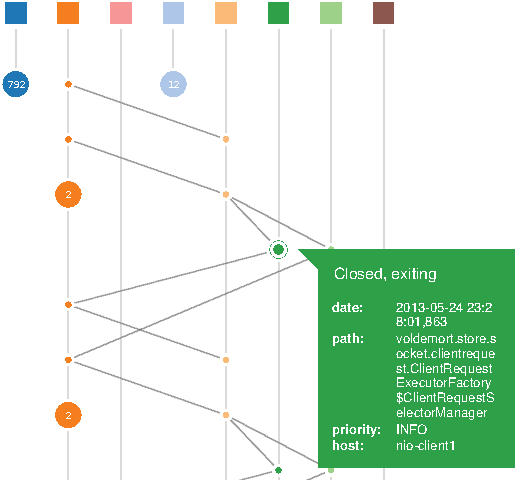
\includegraphics[width=\linewidth]{img/shiviz_time_space.pdf}
	\caption{Interaktives Raum-Zeit-Diagramm in Shiviz \cite{ShiViz_visual_debugger}}
	\label{fig:shiviz}
\end{figure}

Ein sehr mächtiger visueller Debugger ist Oddity \cite{oddity_graphical_debugger}. Das Tool bietet interaktives Debugging, das in
vielen Aspekten klassischen Debuggern ähnelt, allerdings nur auf Systemebene. Oddity erlaubt es, die Ausführung von einzelnen Knoten
des SUT zu pausieren und den Erhalt einzelner Nachrichten und Events an den Knoten zu kontrollieren, alles in einer graphischen Oberfläche, die den
Zustand des Systems inklusive anstehender Nachrichten und Events darstellt. Ein Screenshot dieser Darstellung ist in Abbildung
\ref{fig:oddity} zu sehen. Oddity erlaubt es außerdem den Systemzustand auf einen früheren Zustand zurückzusetzen und so mehrere
Kontrollflüsse in einer Session zu debuggen. Zusätzlich zu der graphischen Oberfläche, die live den Systemzustand abbildet, kann
Oddity auch Zeit-Raum-Diagramme für Abläufe des Systems generieren.

Bei all diesen Vorzügen hat Oddity zwei große Einschränkungen. Einerseits funktioniert das Tool aktuell nur für Systeme, die als
eine Sammlung von Event Handlern implementiert sind. Andererseits erfordert Oddity erheblichen Aufwand zur Einrichtung, da eine
auf das konkrete SUT zugeschnittene Implementierung einer Oddity API erforderlich ist, die direkt mit dem SUT interagieren kann.
Die erste Einschränkung ist nicht inherent und Woos et. al. \cite{oddity_graphical_debugger} schreiben, dass in Zukunft ohne Probleme weitere
Programmiermodelle unterstützt werden können. Der Einrichtungsaufwand dagegen ist tiefer in der Architektur des Tools verankert und
ist zur Umsetzung der vollen Funktionalität notwendig.

\begin{figure}[H]
	\centering
	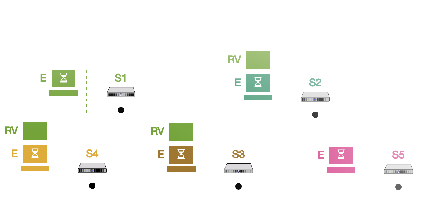
\includegraphics[width=\linewidth]{img/oddity_raft_state.pdf}
	\caption{Visualisierung eines Systemzustands in Oddity \cite{oddity_graphical_debugger}}
	\label{fig:oddity}
\end{figure}

Neben Tools wie ShiViz und Oddity, welche mindestens in ihren jeweiligen akademischen Umfeldern erfolgreich eingesetzt werden
\cite{ShiViz_usage_study, oddity_usage_in_education}, gibt es im Bereich der Visualisierung von verteilten Systemen auch Forschung
zum Einsatz von Augmented Reality. Mit debugAR stellen Reipschläger et. al. \cite{debugAR_AR_debugger} einen Prototypen vor, der
demonstriert, wie Augmented Reality verwendet werden könnte, um die vielen Dimensionen verteilter Systeme zu visualisieren.
Abbildung \ref{fig:debugAR} zeigt ein Rendering von debugAR, dargestellt ist ein interaktives Zeit-Raum-Diagramm ähnlich der
Oberfläche von ShiViz.

\begin{figure}[H]
	\centering
	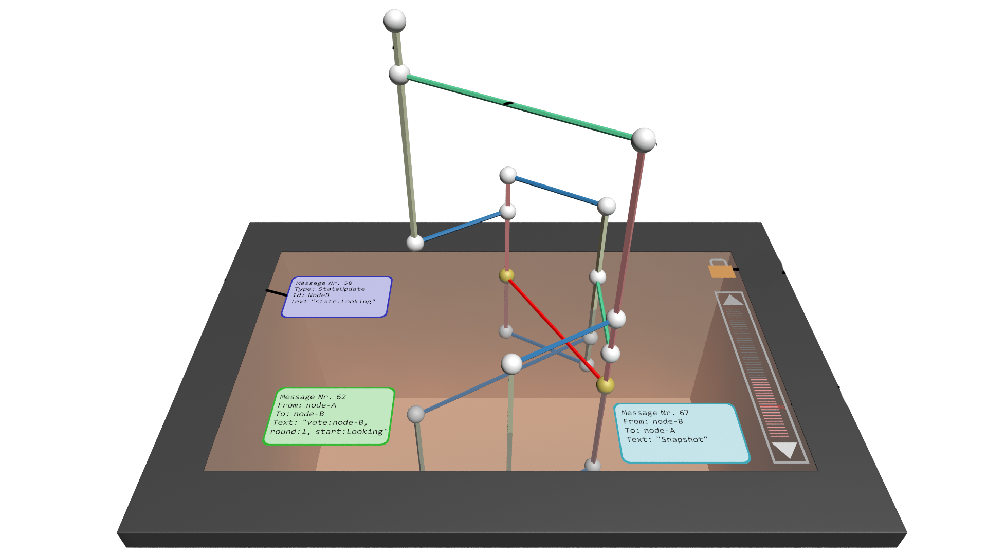
\includegraphics[width=\linewidth]{img/debugAR_rendering.png}
	\caption{Rendering einer 3D Visualisierung von Nachrichtenflüssen in debugAR \cite{debugAR_AR_debugger}}
	\label{fig:debugAR}
\end{figure}

\section{Verwendung von Proxies}
\label{chap:proxies}
Proxies finden in verteilten Systemen unter Anderem Verwendung, um die Verfügbarkeit von Systemen zu verbessern
\cite{distributed_systems_concepts_and_design}, aber auch zum Testen und beim Debugging können Proxies eingesetzt werden. Der bei
Shopify entwickelte Toxiproxy\footnote{\label{foot:toxiproxy}\url{https://github.com/Shopify/toxiproxy}} ist ein für das
Failure-Testing von verteilten Systemen entwickelter TCP-Proxy, welcher Netzwerk-Unterbrechungen und andere Netzwerk-Fehler
simulieren kann.

In anderen Feldern werden Proxies außerdem erfolgreich an verschiedenen Stellen eingesetzt, um Replays von Netzwerk-Verkehr
abzuspielen. Beispielsweise werden Proxy-basierte Replays für reproduzierbare Performance-Tests von nicht-verteilten Systemen
verwendet \cite{performace_replay_testing}. Das Web-Security-Testing-Tool Burp Suite\footnote{\url{https://portswigger.net/burp}}
verwendet ebenfalls einen Proxy, um Requests abzufangen, aufzuzeichnen und gegen ein Angriffziel wiedergeben zu können.

Auch Debugger, die auf das Prinzip setzen, gibt es bereits. Mugshot \cite{mugshot_js_replay_proxy} und ähnliche Tools
\cite{mahimahi_http_replay} sind Replay-Debugger für Browser-Applikationen, die einen Proxy einsetzen, um Requests aufzuzeichnen
und in Replays deterministisch wiederzugeben. Speziell für das Debugging verteilter Systeme wurde ein Proxy-basierter
Replay-Mechanismus hingegen noch nicht eingesetzt.

\section{Offene Fragen und Herausforderungen}
\label{chap:hypothesis}
Fehlertoleranz und Debugging in verteilten Systemen sind aktuelle Forschungsfelder, die sich schnell weiterentwickeln und
dementsprechend noch viele Möglichkeiten für Innovationen bieten. Die folgenden sind derzeit offene Probleme, die weiteren
Entwicklungen bedürfen.

Alvaro und Tymon \cite{abstracting_the_geniuses} stellen als großen aktuellen Mangel heraus, dass sowohl Failure-Testing, als auch
Chaos Engineering in ihrer Anwendung so komplex sind, dass die Techniken ausschließlich den Entwicklern zur Verfügung stehen, die
sich voll darauf spezialisieren. Sie schlagen unter Anderem eine weitgehende Automatisierung von Failure-Testing in der Zukunft
vor. Laut Balalaie et. al. \cite{failify_masters_thesis} fehlt der Industrie außerdem ein Failure-Testing Framework, das es
ermöglicht, effektiv Bugs aufzudecken und diese Bugs mit deterministischen Testfällen zu reproduzieren. Jepsen beispielsweise
agiert ausschließlich zufallsbasiert und kann Bugs oft nicht zuverlässig reproduzieren. Es ist zudem wichtig, dass ein solches
Framework cross-Plattform und Programmiersprachen-agnostisch ist, um weitreichend einsetzbar zu sein. Heute verwenden einige große
Projekte selbst entwickelte Test-Frameworks, die sich auf ein konkretes System beschränken und durch den getrennten
Entwicklungsaufwand nicht mit dem Funktionsumfang von Tools wie Jepsen mithalten können \cite{failify_masters_thesis}.

Im Bereich des Debuggings von verteilten Systemen stellt sich unter Anderem noch die Frage danach, wie unterschiedliche Aspekte
von verteilten Systemen am besten visualisiert werden können \cite{oddity_graphical_debugger}. Auch ist noch offen, wie
interaktive Debugger mit sehr großen Systemen skalieren können, sowohl im Sinne der Visualisierung, als auch der Performance
\cite{gotcha_interactive_debugger}.

Im Kontext ihres Prädikat-Checkers D3S stellen Liu et. al. \cite{d3s_predicate_checker}
insbesondere Replay-Debugging als Teil ihrer Zukunftsvision heraus, um mit D3S identifizierte Bugs einfach zu debuggen. In der
Praxis haben sich seitdem Failure-Testing und Chaos-Engineering gegenüber Prädikat-Checkern zur Bug-Identifikation durchgesetzt.
Nichts desto trotz könnte sich ein Programmiersprachen-agnostischer Replay-Debugger, welcher durch Failure-Testing gefundene Bugs
deterministisch wiedergeben kann, als sehr hilfreich erweisen und ist eine Entwicklung, die es noch zu machen gilt.
In Anbetracht dessen, dass Proxies sich in anderen Bereichen als effektives Werkzeug für Replays von Netzwerk-Verkehr erwiesen
haben (siehe Kapitel \ref{chap:proxies}), scheint es möglich, dass ein Proxy-basierter Replay-Mechanismus der Schlüssel für die
Entwicklung eines solchen Tools sein könnte.

Diese Arbeit stellt die Hypothese auf, dass ein Proxy-basierter Replay-Mechanismus ein effektives Tool beim Debugging von durch
Netzwerk-Unterbrechungen ausgelösten Bugs in verteilten Systemen ist. Ziel ist es, einen Prototypen zu entwickeln, anhand dessen
diese Hypothese evaluiert werden kann. Insbesondere soll empirisch untersucht werden, ob durch Netzwerk-Unterbrechungen ausgelöste
Bugs mit Hilfe eines Proxys in einer Testumgebung deterministisch reproduziert werden können.



\chapter{Ein Proxy zum Debuggen von Netzwerk-Unterbrechungen}
\label{chap:system}
% Dieses Kapitel beschreibt die Idee, die Anforderungen und die Umsetzung des im Rahmen dieser Arbeit entwickelten Systems ditm.
% 
% \section{Idee}
% \label{chap:idea}
Die grundlegende Idee dieser Arbeit ist, einen Proxy als Kernstück eines Replay-Debuggers für verteilte Systeme zu verwenden.
Dieses Kapitel beschreibt die Anforderungen und die Umsetzung des im Rahmen dieser Arbeit entwickelten Prototypen ditm (Debugger
in the middle), anhand dessen das Konzept evaluiert wird.

Grundsätzlich ähnelt ditm dem in Kapitel \ref{chap:proxies} beschriebenen Toxiproxy, der als Failure-Testing-Tool konzipiert ist
in der Hinsicht, dass auch ditm die Möglichkeit bietet, mittels eines Proxies Netzwerk-Unterbrechungen zu erzeugen. Im Gegensatz
zu Failure-Testing-Tools wie dem Toxiproxy geschieht das mit ditm allerdings, während der Nutzer mit dem System interagiert,
anstatt in programmatisch vordefinierten Testfällen. ditm ähnelt in der Hinsicht mehr einem Debugger, als einem Test-Framwork. Um
gefundene Bugs dennoch zuverlässig und mit geringem Aufwand reproduzieren zu können, soll ditm Situationen aufzeichnen und zum
späteren Zeitpunkt wieder abspielen können, insbesondere mit den gleichen Netzwerk-Bedingungen wie während der Aufzeichnung.

% Ein großer Fokus der Arbeit liegt dabei speziell auf dem verfolgten Ansatz für ein solches System. Dieser ist, alle Nachrichten
% innerhalb des SUT über einen Proxy zu leiten, der diese inklusive Metadaten aufzeichnet und in der Lage ist, kontrolliert
% Netwerk-Unterbrechungen zu erzeugen, indem einzelne Nachrichten geblockt, bzw. nicht weiter geleitet, werden. Mit diesem Aufbau
% soll auch ein Replay der Netzwerk-Bedingungen anhand eines zuvor durch den Proxy aufgezeichneten Test-Durchlaufs möglich sein.
% Dazu soll der Proxy während eines Replays für jeden erhaltenen Request identifizieren, welchem Request aus der Aufzeichnung dieser
% entspricht, um die gleichen Netzwerk-Bedingungen erzeugen zu können. Zudem muss der Proxy Requests, die in der Aufzeichnung von
% außerhalb des Systems kommen, identifizieren und während des Replays zum richtigen Zeitpunkt selbstständig an das System senden,
% um so die Interaktionen des Nutzers mit dem System wiederzugeben.

\section{Anforderungen}
ditm ist ein Prototyp, der primär dem Zweck dient, die in Kapitel \ref{chap:hypothesis} aufgestellte Hypothese zu untersuchen.
Die Anforderung reflektieren diesen Umstand, indem beispielsweise ausschließlich HTTP als Netwerk-Protokoll unterstützt wird,
um die Entwicklung einfach zu halten.

\subsection{Funktionale Anforderungen}
Tabelle \ref{tab:fa} beschreibt die funktionalen Anforderungen an das System ditm.
\begin{longtable}[H]{|p{\dimexpr 0.17\linewidth - 6\tabcolsep}|p{0.3\linewidth}|p{0.53\linewidth}|}
	\caption{Funktionale Anforderungen an ditm\label{tab:fa}}                                                                                                                                                                                                                                                                                                                                                                                        \\
	\hline
	ID   & Anforderung                   & Beschreibung                                                                                                                                                                                                                                                                                                                                                                                              \\ \hline
	FA1  & Netzwerk-Unterbrechungen      & Das System soll kontrolliert Netzwerk-Unterbrechungen zwischen Knoten des zu testenden Systems erzeugen können.                                                                                                                                                                                                                                                                                           \\ \hline
	FA2  & Aufzeichnung                  & Das System soll den gesamten Netzwerkverkehr des zu testenden Systems aufzeichnen können. Insbesondere sollen auch erzeugte Netzwerk-Unterbrechungen aufgezeichnet werden.                                                                                                                                                                                                                                \\ \hline
	FA3  & Replay                        & Das System soll anhand einer durch das System erstellten Aufzeichnung die Situation in der Aufzeichnung am laufenden Testsystem wiederherstellen und vor allem inklusive Netzwerk-Unterbrechungen wieder abspielen können. Dabei sollen immer genau die Teile des Netzwerkverkehrs geblockt werden, die auch in der Aufzeichnung vom System geblockt wurden. Nicht mehr, nicht weniger und keine anderen. \\ \hline
	FA4  & Zufällige Unterbrechungen     & Das System soll Netwerk-Unterbrechungen zufällig erzeugen können.                                                                                                                                                                                                                                                                                                                                         \\ \hline
	FA5  & Kontrollierte Unterbrechungen & Das System soll dem Nutzer die Möglichkeit geben, Netwerk-Unterbrechungen feingranular zu steuern.                                                                                                                                                                                                                                                                                                        \\ \hline
	FA6  & Log-Aggregation               & Das System soll zusätzlich zum Netzwerkverkehr auch die Log ausgaben des zu testenden Systems aufzeichnen und aggregieren können.                                                                                                                                                                                                                                                                         \\ \hline
	FA7  & Log-Matching                  & Das System soll die aufgezeichneten Nachrichten und Logs in chronologischer Reihenfolge gemeinsam anzeigen können.                                                                                                                                                                                                                                                                                        \\ \hline
	FA8  & Volume-Snapshots              & Das System soll für zustandsbehaftete Systeme Snapshots der Docker-Volumes erstellen und zu einem späteren Zeitpunk wiederherstellen können, um deterministisch Replays für zustandbehaftete Systeme zu ermöglichen.                                                                                                                                                                                      \\ \hline
	FA9  & Nachrichten von außen         & Das System soll dem Nutzer Schnittstelle bieten, über die Nachrichten reproduzierbar von außen in das zu testende System gesendet werden können, um Prozesse im zu testenden System anzustoßen.                                                                                                                                                                                                           \\ \hline
	FA10 & Responses Blocken             & Das System soll in der Lage sein, nicht nur Requests auf dem Hinweg zum Server zu blockieren, sondern optional auch erst die Antwort auf dem Rückweg.                                                                                                                                                                                                                                                     \\ \hline
\end{longtable}

\subsection{Nicht-Funktionale Anforderungen}
Tabelle \ref{tab:nfa} beschreibt die nicht-funktionalen Anforderungen an das System ditm.
\begin{longtable}[H]{|p{\dimexpr 0.17\linewidth - 6\tabcolsep}|p{0.3\linewidth}|p{0.53\linewidth}|}
	\caption{Nicht-Funktionale Anforderungen an ditm\label{tab:nfa}}                                                                                                                      \\
	\hline
	ID   & Anforderung       & Beschreibung                                                                                                                                               \\ \hline
	NFA1 & Portabilität      & Das System soll vollständig in Docker lauffähig und mittlels docker-compose konfigurierbar sein.                                                           \\ \hline
	NFA2 & Proxy Architektur & Das System soll auf einen Proxy-basierten Replay-Mechanismus setzen, um die in Kapitel \ref{chap:hypothesis} beschriebene Hypothese untersuchen zu können. \\ \hline
	NFA3 & HTTP              & Das System soll mit HTTP als Netzwerkprotokoll arbeiten und grundlegend alle verteilten Systeme, die ausschließlich über HTTP kommunizieren, unterstützen. \\ \hline
	NFA4 & Usability         & Das System soll einfach über eine graphische Oberfläche bedienbar sein.                                                                                    \\ \hline
	NFA5 & Echtzeit          & Requests und Logs einer laufenden Aufzeichnung sollen in Echtzeit angezeigt werden.                                                                        \\ \hline
	NFA6 & Unverändertes SUT & Das SUT soll für die Verwendung des Systems nicht angepasst werden müssen.                                                                                 \\ \hline
\end{longtable}

\section{Architektur}
Das Herzstück des Systems ist entsprechend der Idee ein eigens entwickelter HTTP-Proxy, welcher den Netzwerk-Verkehr in einem
verteilten System inklusive Metadaten aufzeichnet und Nachrichten wahlweise nicht weiter leiten kann, um Netzwerk-Unterbrechungen
zu simulieren. Dieser Proxy läuft in einem Docker Container direkt neben dem SUT und ist auch Teil des gleichen Docker Netzwerks
wie das SUT. Außer dem Proxy hat ditm eine weitere, selbst entwickelte Komponente, ein Log-Driver-Plugin für Docker, welches
Container-Logs an den Proxy sendet. Die Datenflüsse zwischen Komponenten des Systems sind in Abbildung \ref{fig:dataflow} im
Kontext eines SUT mit zwei Knoten dargestellt.
\begin{figure}[H]
	\centering
	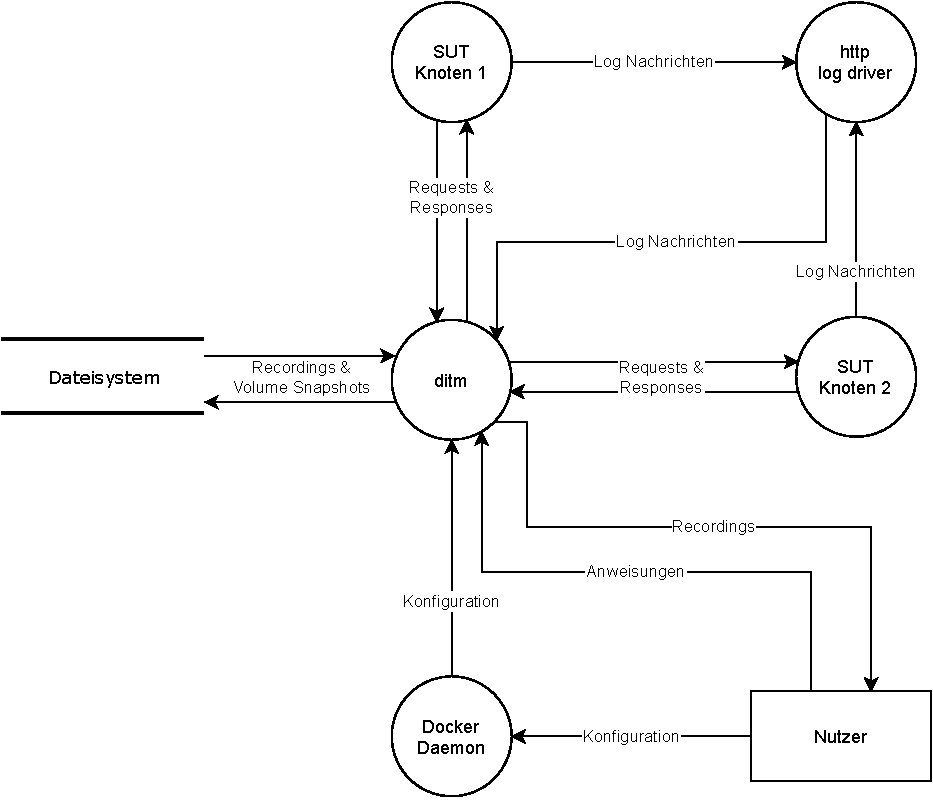
\includegraphics[width=\linewidth]{img/ditm-Dataflow.pdf}
	\caption{Datenflussdiagramm für ditm}
	\label{fig:dataflow}
\end{figure}

\subsection{Datenmodell}
Das Datenmodell von ditm ist einfach gehalten. Das Top Level Datenobjekt ist das Recording, dieses enthält drei chronologisch
geordnete Listen, eine mit den Log Nachrichten des SUT, eine mit den aufgezeichneten Requests und eine mit BlockConfigs, die die
konfigurierten Netzwerk-Unterbrechungen enthalten. Alle Listen enthalten die jeweiligen Objekte für alle Knoten des SUT, ohne
diese weiter voneinander zu trennen. Sollte eine gefilterte Liste benötigt werden, die nur Objekte für bestimmte Knoten enthält,
wird diese dynamisch erzeugt. Recordings enthalten außerdem eine Referenz auf einen Volume Snapshot, sofern für das Recording
einer existiert.

Die eigentlichen Request-Datenobjekte enthalten neben dem Request Body eine Menge Metadaten, die teilweise vom Request selbst
stammen und teilweise durch ditm erzeugt wurden, beispielsweise ob der Request geblockt wurde oder nicht.
Log-Nachrichten umfassen neben der eigentlichen Nachricht ebenfalls wichtige Metadaten, wie den Namen des Containers, der die
Nachricht geloggt hat. In Abbildung \ref{fig:class} ist das beschriebene Datenmodell in einem Klassendiagramm dargestellt. Die
Implementierungen des Matcher-Interfaces fehlen im Klassendiagramm, da sich hier keine Unterschiede zwischen den einzelnen
Implementierungen zeigen würden und diese gesondert in Kapitel \ref{chap:matcher} behandelt werden. Die Methoden der Klasse Proxy wurden
ebenfalls aus Platzgründen weg gelassen und da diese hier konkret von geringerem Interesse sind. Ein Proxy nimmt im Prototypen die
Rolle eines Gottobjekts ein, dieses Design-Pattern wurde für den Prototypen solideren Patterns vorgezogen, um die Entwicklung
einfach zu halten und Erweiterungen, bzw. Änderungen des Datenmodells währenddessen zu erleichtern.
\begin{figure}[H]
	\centering
	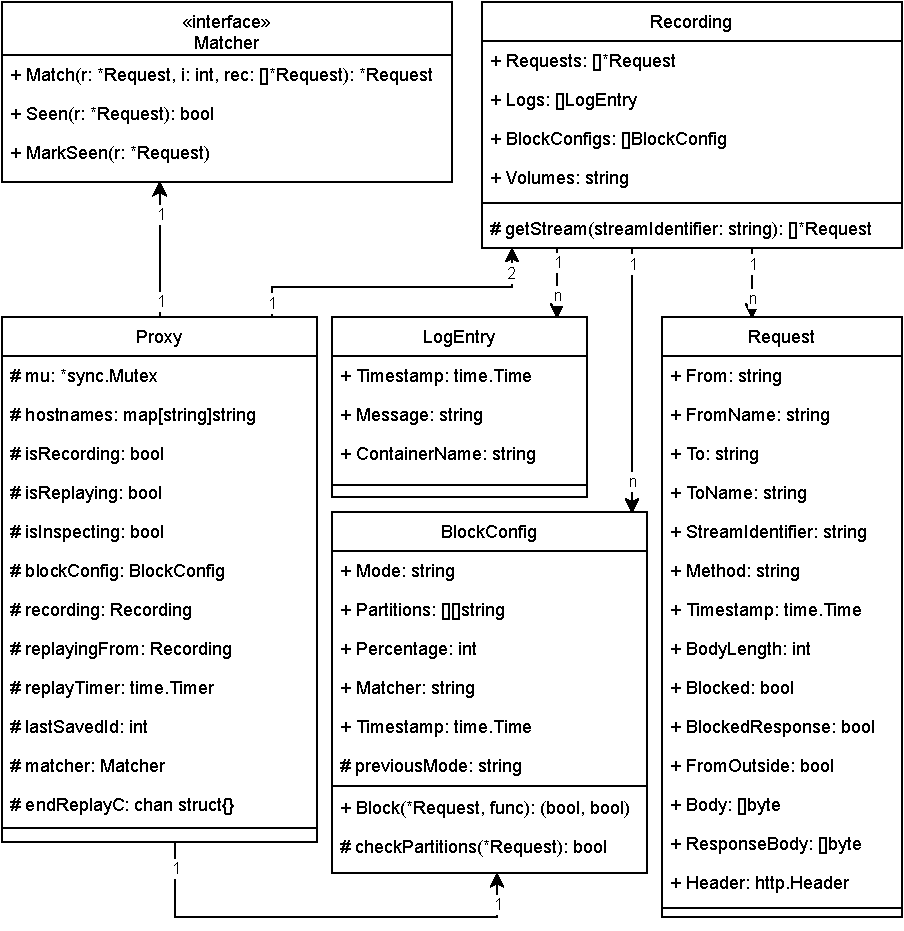
\includegraphics[width=\linewidth]{img/ditm-Class.pdf}
	\caption{Klassendiagramm für ditm ohne Proxy-Methoden und Matcher-Implementierungen}
	\label{fig:class}
\end{figure}

\subsection{Weg eines Requests}
Um eine konkrete Vorstellung von der Arbeitsweise des Proxys zu vermitteln, wird im folgenden beispielhaft der Weg eines
Requests durch das System beschrieben. In diesem Kontext wird der Ursprung des Requests als Client und das Ziel des
Requests als Server bezeichnet, beide sind Knoten des SUT. Abbildung \ref{fig:activity} stellt zunächst den groben Ablauf auf Systemebene dar.
Wichtig ist zu bemerken, dass der Proxy bereits beim ersten erhalten des Requests die komplette Analyse durchführt und
nicht nur entscheidet, ob der Request geblockt werden soll, sondern die Entscheidung auch direkt für die Response trifft,
ohne die Response jemals gesehen zu haben. Tatsächlich wird die Response gar nicht von ditm betrachtet, stattdessen wird
die Analyse vollständig am Request durchgeführt. Die einzige Interaktion des Proxys mit der Response ist, diese zur Anzeige im
Frontend aufzuzeichnen, sie zu blocken falls vorher festgelegt oder sie ansonsten direkt weiter zu leiten.
Der Grund dafür ist, dass fast alle für ditm relevanten Metadaten bereits aus dem Request abgeleitet werden können. Zwar
könnten die Länge der Response und die Response Header möglicherweise ebenfalls von Interesse sein, der Kompromiss wird
hier aber in Kauf genommen, da das die Implementierung erheblich vereinfacht und auch so genügend Metadaten vorliegen,
um verschiedene Algorithmen zur Entscheidung, ob ein Requests im Replay geblockt werden soll, zu evaluieren.
Die verschiedenen Ansätze, die diese Arbeit betrachtet, werden in Kapitel \ref{chap:matcher} behandelt.
\begin{figure}[H]
	\centering
	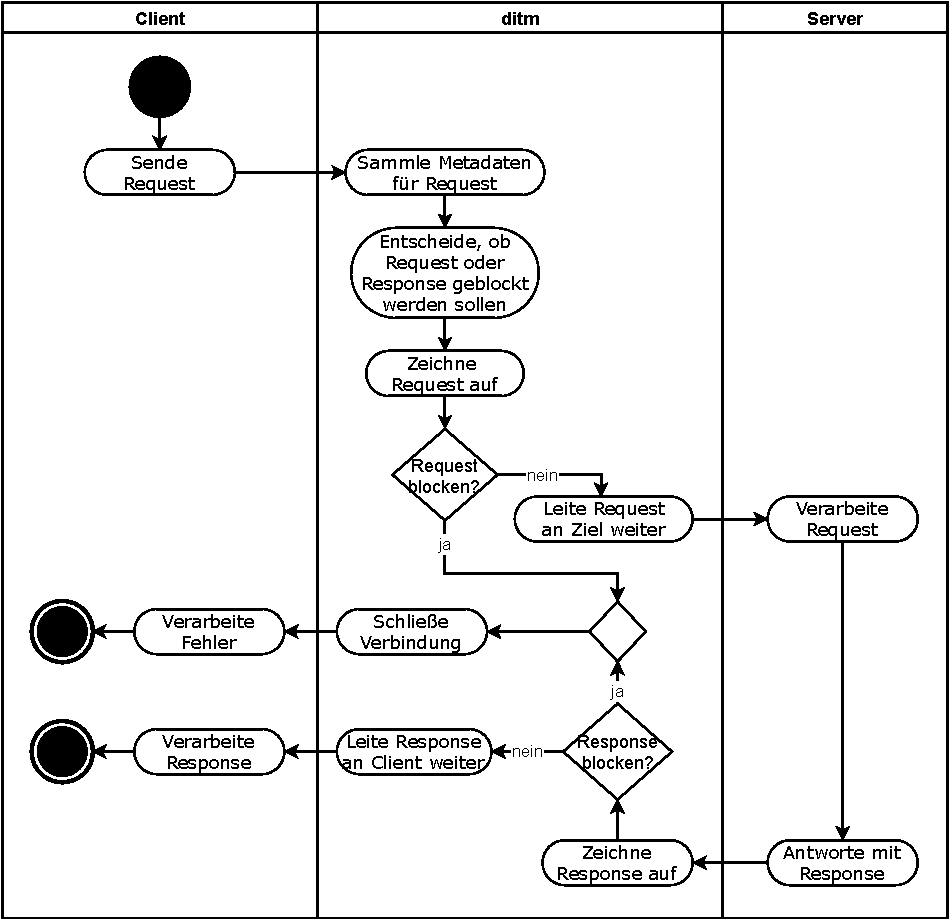
\includegraphics[width=\linewidth]{img/ditm-Activity.pdf}
	\caption{Aktivitätsdiagramm der Interaktion von ditm mit Client und Server eines Requests}
	\label{fig:activity}
\end{figure}

\section{Implementierung}
Als Programmiersprache wird für die Implementierung auf Go gesetzt. Go bietet sich an, da die Standartbibliothek
umfassende, robuste APIs für den Umgang mit Netzwerken bietet und die Sprache insgesamt eine schnelle
Entwicklungsgeschwindigkeit erlaubt, ohne Performance zu vernachlässigen.
\subsection{Datenspeicherung}
Als Speicherformat für ditm wurden einfache Dateien in JSON Format gewählt. So wird jedes Recording Datenobjekt in
einer eigenen Datei serialisiert gespeichert. Dieses Format wurde einer Datenbank aus mehreren Gründen vorgezogen.
Zum einen wird Dateispeicher sowieso für die Volume Snapshots benötigt, die als Zip Dateien gespeichert werden,
es spart also an Komplexität für den Prototypen, für die restlichen Daten ein ähnliches Speichermodel zu wählen.
Zum anderen bieten Dateien den Vorteil, dass der Nutzer die Möglichkeit hat, diese selbst einzeln zu verwalten.
Es ist dem Nutzer also möglich, die Dateien einer einzelnen Aufzeichnung und des zugehörigen Snapshots getrennt
zu sichern oder einfach mit anderen Nutzern über einen generischen Filesharing Dienst zu teilen.
\subsection{Log-Driver}
Um die Log-Ausgaben des SUT in ditm aggregieren zu können, muss ditm aus seinem Container heraus auf die Logs der
anderen Container zugreifen. Leider bietet Docker von sich aus keine einfache Möglichkeit dies zu konfigurieren,
stattdessen muss auf Dockers Plugin-API zurück gegriffen werden. Immerhin bietet Docker eine spezielle Plugin-API
für Log-Driver, die es ermöglicht, Log-Nachrichten durch einen eigenen Driver beliebig weiter zu verarbeiten.
ditm verwendet ein einfaches, eigenes Log-Driver-Plugin, welches Nachrichten als HTTP Request an eine beliebige URL
sendet. ditm selbst bietet in seiner API einen Endpunkt an, welcher diese Log Nachrichten empfangen und verarbeiten kann.
\subsection{Frontend}
Als Frontend bietet ditm dem Nutzer eine Web-Oberfläche, in der laufende sowie vergangene Aufzeichnungen tabellarisch visualisiert
werden können. Des Weiteren ist der Proxy vollständig über die GUI kontrollierbar. Events einer laufenden Aufzeichnung werden in
Echtzeicht per Server-Sent-Events (SSE) an das Frontend gesendet und dort dargestellt. Das Frontend selbst ist eine einfache,
serverseitig gerenderte, HTML-Seite mit dem notwendigen JavaScript Code, um SSEs zu empfangen und zu verarbeiten. Die Seite ist
mittels Bootstrap gestyled und in Tabs aufgeteilt.
\subsection{Request Matcher}
\label{chap:matcher}
Die Logik zur Entscheidung, ob ein Request, bzw. eine Response, während eines Replays geblockt werden soll,
ist ein Kernstück des Proxys, welches es ermöglicht, Aufzeichnungen zuverlässig wiederzugeben.
Das Problem lässt sich darauf herunterbrechen, genau den Request im ursprünglichen Recording zu identifizieren,
dem der aktuelle Request während des Replays entspricht. Das liegt daran, dass sich der Proxy während eines
Replays immer exakt wie während der Aufnahme verhalten soll.

Der erste Schritt dabei, Requests aus Recording und Replay zu matchen, ist immer die Requests sowohl im
Recording als auch im Replay nach dem StreamIdentifier des aktuellen Requests zu filtern, sodass zwei
kleinere Request Streams entstehen. Der StreamIdentifier wird zusammengesetzt aus den Namen des Clients
und des Servers für den jeweiligen Request, ein so gefilterter Stream stellt also den gesamten Verkehr
zwischen genau zwei Knoten des SUT dar.
Der Rest des Matchings ist wie folgt über ein Interface abstrahiert, um leicht mehrere Implementierungen
austauschen zu können.
\begin{lstlisting}
type Matcher interface {
   	Match(r *Request, i int, rec []*Request) *Request
   	Seen(r *Request) bool
    MarkSeen(r *Request)
}
\end{lstlisting}
Die Methode Match erwartet als Parameter den aktuellen Request, dessen Index im gefilterten Stream des Replays
und den gesamten gefilterten Stream des Recordings und gibt einen Pointer auf den Request im Recording zurück,
der das beste Match darstellt. Die Methoden Seen und MarkSeen dienen dazu, Requests zu markieren, falls sie bereits
im aktuellen Replay vorgekommen sind, bzw. abzufragen, ob ein Request bereits markiert wurde. Es wird also nach jedem Aufruf
von Match der zurückgegebene Request markiert. Eine Methode um Requests zu entmarkieren wird nicht benötigt, da für
jedes Replay ein neuer Matcher initialisiert wird. Insgesamt wurden vier Implementierungen für das Interface mit
verschiedenen Algorithmen für Match erstellt, die im Folgenden dargestellt und später gegeneinander evaluiert werden.
Alle vier Implementierungen verwenden eine Hashtabelle zur Umsetzung der Seen und MarkSeen Funktionalität und ignorieren
bei jedem Aufruf von Match bereits markierte Requests, sowie Requests, die von außerhalt des SUT stammen.

\subsubsection{Zählend}
Mit Abstand der einfachste Request-Matcher ist der zählende Matcher. Dieser bestimmt Matches allein aufgrund der Position
von Requests in den jeweiligen Streams. Es wird also immer der Request als Match bestimmt, welcher im Recording den Index i hat,
wobei i der zweite Parameter der Match Methode ist. Ist der entsprechende Request bereits markiert oder von außerhalb des SUT,
wird kein Match zurück gegeben, was bei allen Matchern dazu führt, dass ditm den Request nicht manipuliert.
Der Zählende Matcher ist nicht als ernsthafter Versuch gemeint, einen guten Matcher zu entwickeln. Vielmehr soll
er als Vergleichsgrundlage für die anderen Matcher dienen.

\subsubsection{Exakt}
Alle weiteren Matcher, der exakte eingeschlossen, verwenden ein Punktesystem, in dem allen Requests des Recordings für verschiedene
Eigenschaften Punkte zugewiesen werden und am Ende der Request mit der höchsten Punktzahl als Match zurück gegeben wird.
Der Exakte Matcher vergibt einen Punkt, falls die Requests an gleicher Stelle in ihren Streams stehen, falls die URIs der
Requests gleich sind, falls die Länge der URIs gleich ist, falls die Bodies gleich sind und falls die Länge der Bodies gleich ist.
Sei i der Index im Replay, j der Index im Recording, req der aktuelle Request im Replay und r der aktuelle
Request im Recording, dann wird der Score für r also wie folgt berechnet.
\begin{lstlisting}
score := 0.0
if i == j {
    score += 1
}
if req.To == r.To {
    score += 1
}
if len(req.To) == len(r.To) {
    score += 1
}
if string(req.Body) == string(r.Body) {
    score += 1
}
if len(req.Body) == len(r.Body) {
    score += 1
}
\end{lstlisting}
Dieser Matcher sollte sich in Situationen mit gemischten Request Reihenfolgen bereits deutlich besser verhalten, als der
einfache zählende Matcher, da er neben der Reihenfolge auch andere Eigenschaften der Requests betrachtet. Trotzdem ist es auch
hier vorstellbar, dass der Matcher deutliche Probleme haben wird, sobald er auf eine Menge ähnlicher Requests trifft, die nur
leicht gemischt sind.

\subsubsection{Mix}
Um dieses Problem noch weiter anzugehen, betrachtet der Mix Matcher nicht nur, ob die Position der Requests absolut gleich
ist, sondern den relativen Abstand der Requests zueinander, und bewertet Requests mit geringerem Abstand besser. Alle
anderen Eigentschaften werden weiterhin absolut miteinander verglichen. Um die Gewichtung zwischen dem relativen Abstand
und den konstanten Komponenten des Scores anzupassen, werden diese mit der Länge des Recordings als Faktor multipliziert.
Das führt dazu, dass Gleichheit in anderen Eigenschaften höher gewichtet wird, als die Position eines Requests und diese
nur dann mit ins Gewicht fällt, wenn es mehrere Requests im Recording gibt, die ansonsten gleich gut passen.
\begin{lstlisting}
faktor := float64(len(rec)) // Laenge des Recordings
score := 0.0
score -= math.Abs(float64(j - i)) // Abstand der Requests
if req.To == r.To {
    score += 1 * faktor
}
if len(req.To) == len(r.To) {
    score += 1 * faktor
}
if string(req.Body) == string(r.Body) {
    score += 1 * faktor
}
if len(req.Body) == len(r.Body) {
    score += 1 * faktor
}
\end{lstlisting}

\subsubsection{Heuristisch}
Der Heuristische Matcher unterscheidet sich vom Mix Matcher nur an zwei Stellen. Anstatt die Längen der URIs und Bodies
absolut miteinander zu vergleichen, wird hier wie bei der Position die Differenz zwischen den beiden genommen und eine kleinere
Differenz besser bewertet. Die Werte werden weiterhing mit der Länge des Recordings als Faktor multipliziert. Um die Tatsache
auszugleichen, dass die Differenz selbst größere Werte annehmen kann, als die konstanten Werte, wird sie allerdings zusätzlich
durch 10 dividiert.
\begin{lstlisting}
faktor := float64(len(rec))
score := 0.0
score -= math.Abs(float64(j - i))
if req.To == r.To {
    score += 1 * faktor
}
score -= math.Abs(
    float64(len(req.To)-len(r.To))
) * faktor / 10
if string(req.Body) == string(r.Body) {
    score += 1 * faktor
}
score -= math.Abs(
    float64(len(req.Body)-len(r.Body))
) * faktor / 10
\end{lstlisting}
Obwohl der heuristische Matcher komplexer ist, als der Mix Matcher und insgesamt feinere Unterschiede zwischen Requests
berücksichtigen kann, ist nicht von vornherein zu sagen, ob das von Vorteil ist. Unter anderem wird auch diese Frage in
der Evaluation von ditm empirisch angegangen. Es ist durchaus denkbar, dass es auch von der bestimmten Situation abhängt,
welcher Matcher sich besser verhält.

\subsubsection{Zeitbasiert}
Der Zeitbasierte Matcher funktioniert grundlegend anders als die anderen Matcher und passt nicht direkt in das Design des Matcher
Interfaces. Er bricht insbesondere mit der Idee, Requests einander genau zuzuordnen, um zu entscheiden welche Requests geblockt werden.

Der Zeitbasierte Matcher ist entwickelt für Situationen, in denen selbst bei genau gleichen äußeren Bedingungen das SUT in
Aufzeichnung und Replay unterschiedliche Requests sendet. Die Raft Implementierung, welche in Kapitel \ref{chap:raft} beschrieben wird ist ein
Beispiel für ein System, welches inherent Zufallskomponenten verwendet um zu bestimmen, welche Requests wann gesendet werden.
Die Idee hier ist, Requests nicht ein genaues Match zuzuordnen, sondern stattdessen die BlockConfig zu ermitteln, mit welcher der
Request aufgrund seiner Zeitlichen Position im Replay behandelt werden sollte. Sofern ausschließlich Konfigurationen ohne
Zufallskomponente verwendet wurden, kann dies ein effektiver Weg sein, Replays zu erzeugen, die zwar vielleicht nicht eins zu eins der
Aufzeichnung entsprechen, aber trotzdem Bugs zuverlässig reproduzieren.

Zur Umsetzung werden alle Änderungen an der BlockConfig mit Zeitstempel im Recording gespeichert. Anstelle eines gematchten
Requests gibt der Matcher einen neuen Dummy Request zurück, der lediglich die Information enthält, wie der aktuelle Request
behandelt werden soll. Dieser Workaround ist notwendig, um in das Matcher-Interface zu passen. Auch die Funktionalität des
Matchers, Requests zu identifizieren, die bereits im Replay aufgetaucht sind, wird hier über die im Replay vergangene Zeit
implementiert, sodass Requests als bereits gesehen gelten, sobald der Zeitpunkt überschritten ist, an dem sie in der Aufzeichnung
vorkamen. Einzige Ausnahme hierbei sind die Requests von außerhalb des SUTs. Diese werden wie bei den anderen Matchern erst markiert,
wenn sie tatsächlich gesendet wurden, da es wichtig ist, diese während des Replays vollständig wiederzugeben.

\section{Nutzung}
\subsection{Konfiguration}
ditm wird am einfachsten über docker-compose konfiguriert, dort werden Umgebungsvariablen und Docker-Volumes für das SUT und für
ditm selbst gesetzt. Außerdem muss für den vollen Funktionsumfang der HTTP-Log-Driver ebenfalls in docker-compose konfiguriert
werden, ohne diesen fehlt die Aggregation der Log-Nachrichten. Vor der ersten Verwendung muss der Driver außerdem installiert
werden, dies ist möglich, indem das Repository \url{https://github.com/JonathanArns/http-log-driver} gecloned und darin der Befehl
\textbf{make all} ausgeführt wird. Merke, dass in docker-compose nur alle zum Starten nötigen Einstellungen geschehen, alles andere ist Teil
der Benutzeroberfäche. Eine beispielhafte Konfiguration sieht wie folgt aus.
% \begin{lstlisting}[language=yaml]
\begin{lstlisting}
version: "3.9"

services:
  ditm:
    image: ditm
    hostname: ditm
    environment:
      # Liste der SUT Hostnames
      CONTAINER_HOST_NAMES: target,target2  
    volumes:
      # enthaelt alle Volumes der SUT-Container
      - ./volumes:/volumes  
      - ./recordings:/recordings
      - ./snapshots:/snapshots
    ports:
      - "8000:80"    # Browser UI
      - "5000:5000"  # Proxy
    depends_on:
      - target
      - target2
  
  target:
    image: <image>
    hostname: target
    environment: 
      - HTTP_PROXY=ditm:5000
    volumes:
      - ./volumes/target:/volume
    logging:
      driver: jonathanarns/http-log-driver
      options:
        endpoint: http://localhost:8000/log

  target2:
    image: <image>
    hostname: target2
    environment: 
      - HTTP_PROXY=ditm:5000
    volumes:
      - ./volumes/target2:/volume
    logging:
      driver: jonathanarns/http-log-driver
      options:
        endpoint: http://localhost:8000/log
\end{lstlisting}

\subsection{Bedienung}




\chapter{Versuchsaufbaue}
Dieses Kapitel beschreibt die Versuche, mit denen die in Kapitel \ref{chap:hypothesis} aufgestellte Hypothese evaluiert wird.
Konkret sollen die folgenden Fragen über den zuvor beschriebenen Prototypen ditm beantwortet werden.
\begin{enumerate}
	\item Was sind die Grenzen von ditms Request-Matching?
	\item Wie gut funktioniert ditms Log-Matching, bzw. die chronologische Ordnung von Log-Nachrichten relativ zu Requests?
	\item Lassen sich durch Netzwerk-Unterbrechungen ausgelöste Bugs deterministisch mit ditms Replay-Mechanismen reproduzieren?
\end{enumerate}
\section{Request-Matching}
\label{chap:exp_matching}
Ziel dieses Versuchs ist es, die erste Frage zu beantworten.
Der zeitbasierte Matcher wird in diesem Versuch nicht evaluiert, da er aufgrund seiner Funktionsweise schon per Design für die
zufallsbasierten Netzwerk-Unterbrechungen, die für diese Experimente verwendet werden, ungeeignet ist. Stattdessen wird er nur mit
den Versuchen in \ref{chap:debugging_exp} evaluiert.

Das Test System ist ein einfacher HTTP-Server mit zwei Endpunkten. Einer davon löst eine große Menge an Requests aus, der andere
verarbeitet diese. Es wird für den Versuch ein Cluster aus zwei identischen Knoten verwendet, wovon einer die Rolle eines API
Gateways einnimmt, über das von außen der Versuch ausgelöst wird, und der andere die eines dahinter verborgenen Services. Da ditm
den Nachrichtenfluss zwischen zwei Knoten des SUT immer einzeln betrachtet, genügen zwei Knoten aus, um die Grenzen des
Request-Matchings abzustecken.

Die Requests, die der Gateway-Knoten versendet, sind anhand eines Query Parameters eindeutig identifizierbar. Das System versendet
diese in einer Schleife und bietet neben der Anzahl zu versendener Requests verschiedene andere Konfigurationsmöglichkeiten, die
den Strom von Requests beeinflussen. Die Requests können in vollständig fester oder in unterschiedlich stark gemischter
Reihenfolge erfolgen. Wie stark eine Request-Reihenfolge gemischt ist, wird dabei darüber definiert, um wie viele Stellen ein
Request beim Mischen maximal von seiner ursprünglichen Position verschoben werden kann. Sei dies der Mischungsgrad, dann
entspricht ein Mischungsgrad von 0 immer einem vollständig geordneten Nachrichten-Fluss. Für jeden anderen Wert wird der Fluss vor
jeder Ausführung neu zufällig gemischt, sodass ditm die Requests während eines Replays also in anderer Reihenfolge erhält, als
während der Aufzeichnung. Die folgenden Reihenfolgen stellen beispielhaft dar, wie ein Fluss von zehn Requests bei
unterschiedlichen Mischungsgraden angeordnet werden könnte.
\begin{verbatim}
(0): 0 1 2 3 4 5 6 7 8 9
(1): 1 0 2 4 3 6 5 7 9 8
(2): 0 3 2 1 5 6 4 9 7 8
(3): 4 2 1 0 7 3 9 5 6 8
\end{verbatim}
Requests können außerdem optional asynchron erfolgen, was ebenfalls dazu führt dass sie in stark gemischter Reihenfolge und nahezu
gleichzeitig gesendet werden. Zusätzlich besteht Möglichkeit, entweder einfache GET-Requests zu senden, die selben GET-Requests
mit einem Zeitstempel als zusätzlichem Parameter oder POST-Requests mit einem Zeitstempel und einem zusätzlichen Füller im
Request-Body. Der Füller hat eine von drei festen Längen, somit dient die Länge des Request-Bodys als weiteres Merkmal für ditm,
um Requests identifizierbar zu machen. Die Zeitstempel dienen genau umgekehrt dazu, Requests schwieriger identifizierbar zu
machen, indem ditm durch die Zeitstempel die Query Parameter, bzw. die Bodies der Requests nicht mehr einfach direkt miteinander
vergleichen kann, um Requests zu identifizieren.

Zuletzt gibt es die Möglichkeit, für den verwendeten HTTP-Client (Go net/http) die Wiederverwendung von TCP Verbingungen mit Keep-Alive
zu deaktivieren. Dies ist notwendig, da der Client sonst in bestimmten Situationen Retries sendet, was durch diese Einstellung
verhindert werden kann, mehr dazu in Kapitel \ref{chap:debugging_go}.

Für die Evaluation werden einfache GET-Requests, GET-Requests mit Zeitstempel, GET-Requests ohne Keep-Alive, GET-Requests mit
Zeitstempel und ohne Keep-Alive und POST-Requests verwendet. Für jede Art von Request werden Experimente mit fünf
unterschiedlichen Konfigurationen zur Reihenfolge der Requests durchgeführt. Diese sind asynchron, synchron mit fester Reihenfolge
und synchron mit gemischter Reihenfolge mit Mischungsgraden von 1, 2 und 3. Zusätzlich wird jedes Experiment einmal mit 10
Requests und einmal mit 100 Requests durchgeführt.

In jedem Experiment werden 10 voneinander unabhängige Aufzeichnungen erstellt. Von jeder Aufzeichnung wird dann mit jedem der vier
Request-Matcher ein Replay durchgeführt. Für jedes Replay wird anhand von dazu bestimmten Log Ausgaben des SUT bestimmt, wie viele
Requests ditm falsch behandelt hat. Aus diesem Wert wird dann pro Request-Matcher über die 10 erzeugten Replays der Durchschnitt
und der Median der Anzahl der falsch behandelten Requests berechnet. Diese Werte bilden das Ergebnis des jeweiligen Experiments.
Alle Experimente zum Request-Matching werden vollständig automatisiert durchgeführt und ausgewertet.
% (Das Python Script hierfür ist im Repo)

\section{Log-Matching}
\label{chap:exp_logs}
Für die Evaluation des Log-Matchings wird das gleiche SUT verwendet wie für die Experimente zum Request-Matching.
Da die chronologische Darstellung von Logs zwischen den Requests leider nicht so einfach automatisch auswertbar ist, werden
hierfür zusätzliche Experimente von Hand durchgeführt und ausgewertet. Es werden insgesamt vier Experimente durchgeführt, bei
denen eine Aufzeichnung mit jeweils 10 und 100 Requests einmal synchron und einmal asynchron erstellt wird. Das Ergebnis sind
hierbei jeweils zwei Werte: die maximale Entfernung einer Log Nachricht von ihrer korrekten Position, also der größte vorgekommene
Fehler und die Gesamtzahl an Nachrichten, die an falscher Stelle eingeordnet wurden, also die Anzahl vorgekommener Fehlern. Da das
Log-Matching im Replay exakt gleich funktioniert, wie in der Aufzeichnung, sind für die Evaluation des Log-Matchings keine Replays
notwendig.

\section{Debugging}
\label{chap:debugging_exp}
Im Folgenden sollen die tatsächlichen Debugging Möglichkeiten von ditm möglichst empirisch evaluiert werden. Eine empirische
Evaluation eines Debuggers ist grundsätzlich schwierig, da es beim Debugging vor allem darum geht, Entwicklern beim
Verständnis eines komplexen Problems zu helfen, welches sie noch nie zuvor gesehen haben. Es bräuchte also im Optimalfall eine
große Menge relevanter, bekannter Bugs und Entwickler, denen diese Bugs vollständig unbekannt sind, um zu evaluieren, wie effektiv
ein Debugger tatsächlich ist.

Eine solche Studie würde den Rahmen dieser Arbeit bei weitem sprengen. Stattdessen wird hier evaluiert, ob ditm tatächlich in der
Lage ist, Bugs zu finden und deterministisch in Replays reproduzieren. Das ist die Funktionalität, die im Kern dieser Arbeit steht
und die essenziell für das angedachten Debugging-Konzept von ditm ist.

Dazu werden Systeme mit bekannten Bugs verwendet, die durch Netzwerk-Unterbrechungen ausgelöst werden. Die Bugs sollen mit Hilfe
von ditm erst in einer Aufzeichnung nachweislich erzeugt werden und dann wiederholbar in Replays wiedergegeben werden.

\subsection{Systeme}
Es werden insgesamt drei verschiedene Systeme verwendet, in denen jeweils mindestens ein Bug im Zusammenhang mit
Netzwerk-Unterbrechungen bekannt ist.

\subsubsection{Bank}
Das erste System ist eine kleine Bank Simulation mit einem zentralen Server, der Kontodaten transaktionell verwaltet und einem
API-Gateway, welches die Funktionalitäten des Systems kapselt. Es werden insgesamt vier Operationen unterstützt, das Anlegen eines
Kontos, das Abfragen eines Kontostands und das Ein- und Auszahlen von Geld auf einem Konto.

\subsubsection{Raft}
\label{chap:raft}
Das zweite System ist eine Implementierung des Raft-Konsens-Algorithmus in der Form eines Append-Logs. Die Implementierung basiert
auf einem auf Github öffentlichen Hobby-Projekt\footnote{https://github.com/eileen-code4fun/SimpleRaft}, das Raft mit Threads als
Knoten umsetzt. Für diese Arbeit wurde die Implementierung angepasst, um als verteiltes System zu laufen und über HTTP zu
kommunizieren. Obwohl es sich um eine minimale Implementierung handelt, ist diese im Sinne des Raft-Algorithmus vollständig und
bietet damit alle nötige Funktionalität, um daran Bugs aus realen verteilen Systemen, die ähnliche Algorithmen verwenden,
nachstellen zu können. Dazu zählen Systeme wie MongoDB, Redis und VoltDB. Die Bugs, welche hier nachgestellt werden, stammen
ursprünglich aus MongoDB und Redis.

\subsubsection{Startup}
Das dritte und letzte System ist das System eines realen jungen Startups. Konkret handelt es sich um eine SaaS-Lösung für das
Sustainability Reporting von Mittelständischen Unternehmen. Das System setzt auf eine verteilte, Service-orientierte Architektur
und besteht aus derzeit 5 Services. Im Kontext von ditm kann einer der fünf Services nicht verwendet werden, da dieser von AWS
Diensten wie S3 abhängig ist, es wird hier also ein Cluster aus vier Knoten verwendet. Die anderen Services sind von dem
fehlenden Service nicht abhängig und können auch in dieser kleineren Konstellation problemlos funktionieren.

\subsection{Bekannte Bugs}
Hier sind die bekannten Bugs in den jeweiligen Systemen beschrieben, die hier mit Hilfe von ditm untersucht werden sollen.

\subsubsection{B1: Doppelte Buchung}
% ergebnis: funktioniert nur mit heuristic, weil blockconfig optionen im prototypen fehlen
Das Banksystem wurde speziell für dieses Szenario entwickelt und enthält einen Bug, welcher dazu führt, dass Ein- und Auszahlungen
doppelt auf einem Konto verbucht werden können. Konkret tritt dieses Problem auf, weil das API Gateway automatisch Retries für
fehlgeschlagene Operationen sendet und die Ein- und Auszahlung nicht idempotent sind. Um den Bug zu reproduzieren, muss ein Ein-
oder Auszahlungsrequest an das API Gateway gesendet werden und die Response auf den Request zwischen Bankserver und Gateway
von einer Netzwerk-Unterbrechung geblockt werden.

\subsubsection{B2: Dirty Reads in MongoDB}
% ergebnis: funktioniert nur mit timing
Ein Dirty Read ist eine Lese-Operation, die Daten aus Schreiboperationen enthält, die später zurück gerollt werden. Dirty Reads
sind problematisch, weil sie falsche Daten liefern. Eine Schreiboperation, die zurückgerollt wird, ist im Endeffekt niemals
passiert, sie sollte also auch niemals gelesen werden können. \cite{jepsen_mongo_analysis}

\begin{figure}[H]
	\centering
	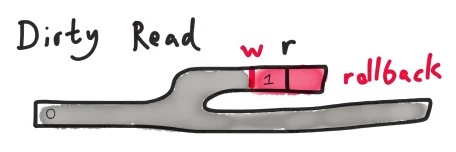
\includegraphics[width=0.7\linewidth]{img/dirty_read.png}
	\caption{Visualisierung eines Dirty Reads. Ist `w` eine Schreiboperation, die später zurückgerollt wird, dann ist `r` ein
		Dirty Read. \cite{jepsen_mongo_analysis}}
	\label{fig:dirty_read}
\end{figure}

Jepsen hat in MongoDB Version 2.6.7 einen Bug entdeckt, der im Fall gewisser Netzwerk-Unterbrechungen für eine kurze Zeit Dirty
Reads zulässt. Wenn der Leader-Knoten von der Mehrheit des Clusters getrennt wird, tritt dieser nach einem Timeout selbst zurück
und nimmt keine Schreiboperationen mehr entgegen. Wird allerdings vor diesem Timeout ein Wert über diesen Leader geschrieben, kann
dieser von dort auch gelesen werden, bevor er später zurückgerollt wird. Das liegt daran, dass in MongoDB damals neue
Schreiboperationen unter allen Konsistenzeinstellungen sofort vom Leader lesbar waren, noch bevor sie an eine Mehrheit des
Clusters repliziert wurden. \cite{jepsen_mongo_analysis}

Dieser Bug wird hier originalgetreu mittels der beschriebenen Raft Implementierung simuliert.

\subsubsection{B3: Election-Endlosschleife in MongoDB}
% ergebnis: funktioniert mit beiden bei 3 knoten (heuristic replay end unzuverlässig), bei mehr nur mit timing
Für die meisten Bugs bei Netzwerk-Unterbrechungen müssen Teile eines verteilten Systems vollständig voneinander getrennt sein. Es
gibt allerdings auch Bugs, die sich nur bei einer teilweisen Zertrennung eines Systems manifestieren. Ein Beispiel, welches
Alquraan et. al. \cite{analysis_of_network_partition_failures} nennen, ist ein Bug in MongoDB, welcher zu einer Schleife führt, in
der endlos neue Leader gewählt werden. MongoDB verwendet einen Verwaltungsknoten, um unentschiedene Elections zu entscheiden.
Tritt in einem Cluster mit zwei Replica-Knoten und einem Verwaltungsknoten eine Netzwerk-Unterbrechung wie in Abbildung
\ref{fig:partial_partition_mongo} auf, führt das dazu, dass Knoten A und B sich abwechselnd zum Leader wählen lassen, da sie jeweils nie
den Leader erreichen können, der Verwaltungsknoten aber immer an beiden Elections teilnehmen kann und den alten Leader dann über
den neuen Leader informiert. Dieser Bug manifestiert sich vollständig ohne Interaktionen durch einen Client von außen und
der Effekt verschwindet wieder, sobald die Netzwerk-Unterbrechung geheilt ist.

\begin{figure}[H]
	\centering
	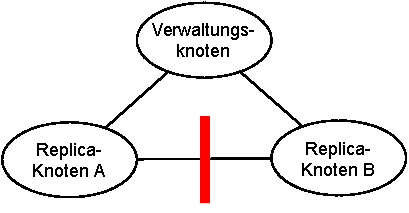
\includegraphics[width=0.6\linewidth]{img/ditm-Partitions.pdf}
	\caption{Visualisierung einer Netzwerk-Unterbrechung (rot), die in MongoDB eine Election-Endlosschleife auslösen konnte}
	\label{fig:partial_partition_mongo}
\end{figure}

Im Gegensatz zu MongoDB verwendet Raft keinen Verwaltungsknoten. Der beschriebene Bug kann dennoch realitätsnah in einem
Raft-Cluster nachgestellt werden, da in Raft jeder Knoten die Rolle einnehmen kann, die in MongoDB der Verwaltungsknoten für diesen
Bug spielt. Dazu müssen in Raft zwei Sicherheitsmechanismen ausgeschaltet werden:
\begin{itemize}
	\item dass Knoten nur für einen Leader gleichzeitig stimmen dürfen und
	\item dass Knoten nur Leader akzeptieren,  die in  wie sie selbst haben.
\end{itemize}

\subsubsection{B4: Split-Brain in Redis-Raft}
% ergebnis: funktioniert nur mit timing
Wenn ein Leader-basiertes System wie Raft mehr als einen Leader-Knoten gleichzeitig hat, wird dies als Split-Brain Situation
bezeichnet. Um diese Situationen zu vermeiden hat Raft verschiedene Sicherheitsmaßnahmen, wie dass jeder Knoten pro Term nur für
einen Leader stimmen darf. Die Maßnahme, dessen Fehlen diesen konkreten Bug ermöglicht, ist, dass das Entfernen eines Knotens aus
dem Cluster eine Mehrheitsentscheidung aller Knoten ist. Der Leader sollte also nicht in der Lage sein, einen Knoten zu entfernen,
ohne eine Bestätigung der Aktion von mindestens der Hälfte des Clusters zu erhalten.

Einer frühen Version der Raft-Implementierung Redis-Raft, welche optinal in Redis verwendet werden kann, fehlte diese
Einschränkung. In dieser Version ist es möglich, eine Split-Brain Situation zu erzeugen, indem der Leader durch eine
Netzwerk-Unterbrechung vom Rest des Clusters getrennt wird und dann auf einmal angewiesen wird, alle anderen Knoten aus dem
Cluster zu entfernen. Das führt dazu, dass der alte Leader effektiv zu einen ein-Knoten Cluster wird, während die anderen Knoten
einen neuen Leader wählen und gemeinsam weiter als Cluster funktionieren. Das passiert, weil die anderen Knoten durch die
Netzwerk-Unterbrechung nie von ihrer Entfernung informiert werden und diese auch nicht bestätigen. \cite{jepsen_redis_raft}

\subsubsection{B5: Unereichbare Daten}
% token login funktioniert in replays nicht, workaround: token lifetime wurde für Experimente auf 100 Tage gesetzt
% ergebnis: funktioniert mit beiden matchern
Das Startup-System verwendet ein eigenes, hierarchie-basiertes Authorisierungssystem. Dieses erlaubt es, Lese- und
Update-Operationen in jedem Service lokal zu authorisieren, für das Anlegen neuer Daten ist aber ein Request an den zentralen
Usermanagement-Service notwendig. Eine frühe Version dieses Authorisierungssystems hatte einen Bug, der dazu führte, dass neu
geschrieben Daten für Nutzer unzugänglich würden, sollte der Usermanagement-Service während der Schreiboperation unerreichbar
sein. Das lag daran, dass die Daten in diesem Fall einfach ohne die zur Authorisierung notwendige ID geschrieben wurden, die vom
Usermanagement-Service kommen sollte.

In neueren Versionen des Systems schlagen stattdessen Schreiboperationen in diesem Fall ganz fehl, um inkonsistente Datenstände zu
verhindern. Der Bug wurde hier in eine aktuelle Version des Systems wieder eingebaut, anstatt die alte Version des Systems zu
verwenden, da dies einfacher war, als kompatible alte Versionen aller Teile des Systems zu finden und zu konfigurieren.



\chapter{Ergebnisse}
\label{chap:results}
Im Folgenden werden die Ergebnisse der einzelnen Experimente dargestellt und interpretiert. Im Anschluss folgt eine
zusammenfassende Diskussion der Evaluationsergebnisse.

\section{Request-Matching}
Die Ergebnisse der Experimente zur Evaluation den Request-Matchings sind gruppiert nach Art der Requests, sodass pro Tabelle
der Einfluss von Zufall in der Reihenfolge der Requests auf das Matching erkennbar wird.
Jede Zeile in den Tabellen stellt die Ergebnisse für eine bestimmte Konfiguration des in Kapitel \ref{chap:exp_matching}
beschriebenen Versuchs dar, jeweils für die vier verschiedenen Request-Matcher, die in den Versuchen evaluiert werden. Für jedes Experiment
wird wowohl der Durchschnitt, als auch der Median über 10 individuelle Durchführungen des jeweiligen Versuchs angegeben.

% Die Erklärung hierfür ist, dass durch den Bug ein vorangegangener Aufruf des SUT einen
% Einfluss auf den nächsten haben kann, falls der letzte Request des vorangegangenen Aufrufs erfolgreich war und der erste Request
% des neuen Aufrufs geblockt wird. In diesem Fall wird der erste Request erneut versucht, was in isolation selbst mit dem Bug
% nicht passieren sollte. Tritt dieser Fall ein, verändert sich dadurch die Reihenfolge des gesamten Request-Flusses, da direkt am
% Anfang ein zusätzlicher Request eingefügt wird, was zu den beobachteten Fehlern führt. Tabelle \ref{tab:get_nka} zeigt, dass
% diese Fehler in der Tat durch den Bug ausgelöst werden, da sie nicht auftreten, wenn die Retries mittels no-keep-alive
% verhindert werden. Des weiteren zeigt sich an den jeweils geringeren Request Anzahlen, dass der Bug deutlich weniger bei den
% asynchronen Experimenten auftritt, vermutlich, weil dort weniger Verbindungen wiederverwendet werden, als im synchronen
% Versuchsaufbau. Das seltenere Auftreten des Bugs erklärt auch die deutlich bessere Performance der heuristischen und Mix-Matcher
% bei den asynchronen Experimenten im Vergleich zu den synchron gemischten in Tabelle \ref{tab:get}.
\begin{table}[H]
	\centering
	\caption{
		Ergebnisse zum Request-Matching von einfachen GET-Requests:
		Anzahl der im Replay falsch behandelten Requests pro Anzahl Requests im Recording,
		beides als Durchschnitt und Median über zehn Durchführungen des Versuchs mit dem jeweiligen Matcher.
	}
	\label{tab:get}
	\begin{tabular}{|l|r|r|r|r|r|r|r|r|r|r|r|}
		\hline
		\multirow{3}{*}{Shuffle} & \multicolumn{2}{|c|}{Anzahl}   & \multicolumn{2}{|c|}{Heurist.} & \multicolumn{2}{|c|}{Exakter} & \multicolumn{2}{|c|}{Mix}     & \multicolumn{2}{|c|}{Zählender}                                    \\
		                         & \multicolumn{2}{|c|}{Requests} & \multicolumn{2}{|c|}{Matcher}  & \multicolumn{2}{|c|}{Matcher} & \multicolumn{2}{|c|}{Matcher} & \multicolumn{2}{|c|}{Matcher}                                      \\ \cline{2-11}
		                         & avg                            & med                            & avg                           & med                           & avg                             & med  & avg  & med  & avg  & med  \\ \hline
		no                       & 13.3                           & 13.5                           & 0.8                           & 0.0                           & 0.8                             & 0.0  & 0.8  & 0.0  & 1.7  & 0.0  \\ \hline
		no                       & 133.6                          & 133.0                          & 2.9                           & 0.0                           & 0.3                             & 0.0  & 2.9  & 0.0  & 15.2 & 0.0  \\ \hline
		1                        & 13                             & 13.0                           & 1.7                           & 1.5                           & 2.2                             & 2.0  & 1.7  & 2.0  & 2.6  & 2.5  \\ \hline
		1                        & 133.2                          & 134.0                          & 22.7                          & 23.0                          & 39.1                            & 38.0 & 23.6 & 25.0 & 34.6 & 36.5 \\ \hline
		2                        & 13.5                           & 14.0                           & 2.5                           & 2.5                           & 3.0                             & 3.0  & 2.5  & 3.0  & 3.3  & 4.0  \\ \hline
		2                        & 131.5                          & 130.0                          & 22.5                          & 21.5                          & 40.3                            & 42.5 & 21.4 & 20.0 & 45.2 & 46.0 \\ \hline
		3                        & 13.3                           & 14.0                           & 2.0                           & 2.0                           & 3.5                             & 3.0  & 2.3  & 2.5  & 4.5  & 4.0  \\ \hline
		3                        & 135.1                          & 137.0                          & 25.8                          & 27.0                          & 42.2                            & 39.0 & 24.8 & 27.5 & 46.7 & 47.0 \\ \hline
		async                    & 13                             & 14.0                           & 1.5                           & 1.5                           & 3.4                             & 4.0  & 1.4  & 1.0  & 5.5  & 5.0  \\ \hline
		async                    & 113.1                          & 111.5                          & 7.2                           & 6.5                           & 30.7                            & 31.0 & 7.0  & 6.0  & 68.2 & 67.0 \\ \hline
	\end{tabular}
\end{table}

Die Tabellen \ref{tab:get} und \ref{tab:get_ts} stellen die Ergebnisse der Experimente dar, in denen durch Retries vom HTTP-Client
mehr Requests gesendet wurden, als die im Versuchsaufbau speziefizierten 10 oder 100. Die zusätzlichen Requests sind in jedem
Aufruf des SUT unterschiedlich, auch zwischen Recordings und deren Replays.

In diesen Experimenten ist zu beobachten, dass selbst bei ungemischten Request-Flüssen mit allen Matchern Fehler in manchen
Replays passieren. Trotzdem ist zu erkennen, dass der Heuristische und der Mix-Matcher sich hier insgesamt deutlich besser
verhalten, als die anderen beiden. In den Versuchen mit Zeitstempeln, deren Ergebnisse in Tabelle \ref{tab:get_ts} dargestellt
sind, machen der Heuristische und der Mix-Matcher in vielen Konfigurationen des Versuchs ein Vielfaches der Fehler, die sie in den
Versuchen ohne Zeitstempel in Tabelle \ref{tab:get} machen.

% Obwohl ein korrektes Request-Matching bei gemischter Reihenfolge durch den Bug effektiv unmöglich wird, da schlichtweg nicht die
% gleichen Requests im Recording und im Replay sind, ist zu erkennen, dass
% Das ist in so fern relevant, dass auch in realen Szenarien durchaus
% unterschiedliche Mengen an Requests in Recording und Replay sein können, beispielsweise wenn im Laufe eines Debugging Workflows
% ein möglicher Bugfix getestet werden soll.
\begin{table}[H]
	\centering
	\caption{
		Ergebnisse zum Request-Matching von GET-Requests mit Zeitstempel:
		Anzahl der im Replay falsch behandelten Requests pro Anzahl Requests im Recording,
		beides als Durchschnitt und Median über zehn Durchführungen des Versuchs mit dem jeweiligen Matcher.
	}
	\label{tab:get_ts}
	\begin{tabular}{|l|r|r|r|r|r|r|r|r|r|r|r|}
		\hline
		\multirow{3}{*}{Shuffle} & \multicolumn{2}{|c|}{Anzahl}   & \multicolumn{2}{|c|}{Heurist.} & \multicolumn{2}{|c|}{Exakter} & \multicolumn{2}{|c|}{Mix}     & \multicolumn{2}{|c|}{Zählender}                                    \\
		                         & \multicolumn{2}{|c|}{Requests} & \multicolumn{2}{|c|}{Matcher}  & \multicolumn{2}{|c|}{Matcher} & \multicolumn{2}{|c|}{Matcher} & \multicolumn{2}{|c|}{Matcher}                                      \\ \cline{2-11}
		                         & avg                            & med                            & avg                           & med                           & avg                             & med  & avg  & med  & avg  & med  \\ \hline
		no                       & 13.6                           & 14.0                           & 0.7                           & 0.0                           & 0.9                             & 0.0  & 1.2  & 0.0  & 2.1  & 0.0  \\ \hline
		no                       & 134.7                          & 136.5                          & 19.6                          & 0.0                           & 19.0                            & 0.0  & 9.4  & 0.0  & 19.9 & 0.0  \\ \hline
		1                        & 13.8                           & 14.0                           & 3.3                           & 3.0                           & 3.0                             & 2.5  & 3.8  & 4.0  & 3.0  & 3.5  \\ \hline
		1                        & 135.4                          & 137.5                          & 37.0                          & 37.0                          & 36.2                            & 35.0 & 36.7 & 36.5 & 38.1 & 39.5 \\ \hline
		2                        & 13.4                           & 13.0                           & 3.7                           & 4.0                           & 4.3                             & 4.5  & 3.2  & 3.5  & 3.4  & 3.0  \\ \hline
		2                        & 134.1                          & 133.5                          & 42.0                          & 41.0                          & 43.1                            & 45.0 & 40.0 & 37.5 & 42.9 & 42.0 \\ \hline
		3                        & 13.2                           & 13.0                           & 4.1                           & 4.0                           & 5.3                             & 6.0  & 5.0  & 6.0  & 4.8  & 5.0  \\ \hline
		3                        & 134.5                          & 134.5                          & 48.8                          & 47.0                          & 48.3                            & 47.5 & 50.8 & 51.5 & 49.1 & 48.0 \\ \hline
		async                    & 13.7                           & 13.5                           & 5.0                           & 5.0                           & 5.6                             & 5.0  & 6.1  & 6.0  & 6.2  & 6.5  \\ \hline
		async                    & 113.4                          & 108.0                          & 60.9                          & 60.0                          & 65.2                            & 65.0 & 65.0 & 65.0 & 65.6 & 66.5 \\ \hline
	\end{tabular}
\end{table}

\begin{table}[H]
	\centering
	\caption{
		Ergebnisse zum Request-Matching von GET-Requests mit no-keep-alive Header:
		Anzahl der im Replay falsch behandelten Requests pro Anzahl Requests im Recording,
		beides als Durchschnitt und Median über zehn Durchführungen des Versuchs mit dem jeweiligen Matcher.
	}
	\label{tab:get_nka}
	\begin{tabular}{|l|r|r|r|r|r|r|r|r|r|r|r|}
		\hline
		\multirow{3}{*}{Shuffle} & \multicolumn{2}{|c|}{Anzahl}   & \multicolumn{2}{|c|}{Heurist.} & \multicolumn{2}{|c|}{Exakter} & \multicolumn{2}{|c|}{Mix}     & \multicolumn{2}{|c|}{Zählender}                                  \\
		                         & \multicolumn{2}{|c|}{Requests} & \multicolumn{2}{|c|}{Matcher}  & \multicolumn{2}{|c|}{Matcher} & \multicolumn{2}{|c|}{Matcher} & \multicolumn{2}{|c|}{Matcher}                                    \\ \cline{2-11}
		                         & avg                            & med                            & avg                           & med                           & avg                             & med  & avg & med & avg  & med  \\ \hline
		no                       & 10                             & 10.0                           & 0.0                           & 0.0                           & 0.0                             & 0.0  & 0.0 & 0.0 & 0.0  & 0.0  \\ \hline
		no                       & 100                            & 100.0                          & 0.0                           & 0.0                           & 0.0                             & 0.0  & 0.0 & 0.0 & 0.0  & 0.0  \\ \hline
		1                        & 10                             & 10.0                           & 0.0                           & 0.0                           & 1.7                             & 2.0  & 0.0 & 0.0 & 4.2  & 3.5  \\ \hline
		1                        & 100                            & 100.0                          & 0.0                           & 0.0                           & 22.5                            & 22.5 & 0.0 & 0.0 & 40.2 & 41.0 \\ \hline
		2                        & 10                             & 10.0                           & 0.0                           & 0.0                           & 2.5                             & 2.0  & 0.0 & 0.0 & 3.6  & 4.0  \\ \hline
		2                        & 100                            & 100.0                          & 0.0                           & 0.0                           & 25.4                            & 25.5 & 0.0 & 0.0 & 48.8 & 50.5 \\ \hline
		3                        & 10                             & 10.0                           & 0.0                           & 0.0                           & 2.2                             & 2.0  & 0.0 & 0.0 & 5.0  & 5.0  \\ \hline
		3                        & 100                            & 100.0                          & 0.0                           & 0.0                           & 25.4                            & 25.0 & 0.0 & 0.0 & 52.2 & 53.0 \\ \hline
		async                    & 10                             & 10.0                           & 0.0                           & 0.0                           & 2.5                             & 2.5  & 0.0 & 0.0 & 7.3  & 7.5  \\ \hline
		async                    & 100                            & 100.0                          & 0.0                           & 0.0                           & 22.4                            & 21.5 & 0.0 & 0.0 & 68.2 & 65.5 \\ \hline
	\end{tabular}
\end{table}

Tabelle \ref{tab:get_nka} zeigt, dass ditm problemlos mit stark gemischten Requests umgehen kann, sofern diese keine weiteren zufälligen
komponenten enthalten. Auch hier verhalten sich der Heutristische und der Mix-Matcher am besten, die beiden anderen
Matcher haben deutliche Probleme.

\begin{table}[H]
	\centering
	\caption{
		Ergebnisse zum Request-Matching von GET-Requests mit Zeitstempel no-keep-alive Header:
		Anzahl der im Replay falsch behandelten Requests pro Anzahl Requests im Recording,
		beides als Durchschnitt und Median über zehn Durchführungen des Versuchs mit dem jeweiligen Matcher.
	}
	\label{tab:get_ts_nka}
	\begin{tabular}{|l|r|r|r|r|r|r|r|r|r|r|r|}
		\hline
		\multirow{3}{*}{Shuffle} & \multicolumn{2}{|c|}{Anzahl}   & \multicolumn{2}{|c|}{Heurist.} & \multicolumn{2}{|c|}{Exakter} & \multicolumn{2}{|c|}{Mix}     & \multicolumn{2}{|c|}{Zählender}                                    \\
		                         & \multicolumn{2}{|c|}{Requests} & \multicolumn{2}{|c|}{Matcher}  & \multicolumn{2}{|c|}{Matcher} & \multicolumn{2}{|c|}{Matcher} & \multicolumn{2}{|c|}{Matcher}                                      \\ \cline{2-11}
		                         & avg                            & med                            & avg                           & med                           & avg                             & med  & avg  & med  & avg  & med  \\ \hline
		no                       & 10                             & 10.0                           & 0.0                           & 0.0                           & 0.0                             & 0.0  & 0.0  & 0.0  & 0.0  & 0.0  \\ \hline
		no                       & 100                            & 100.0                          & 0.0                           & 0.0                           & 0.0                             & 0.0  & 0.0  & 0.0  & 0.0  & 0.0  \\ \hline
		1                        & 10                             & 10.0                           & 3.4                           & 3.0                           & 4.3                             & 4.0  & 3.7  & 4.0  & 3.5  & 3.5  \\ \hline
		1                        & 100                            & 100.0                          & 40.7                          & 39.0                          & 43.8                            & 45.0 & 40.4 & 40.0 & 43.7 & 43.0 \\ \hline
		2                        & 10                             & 10.0                           & 5.3                           & 5.5                           & 4.9                             & 5.0  & 5.0  & 4.5  & 4.4  & 4.0  \\ \hline
		2                        & 100                            & 100.0                          & 50.6                          & 51.5                          & 48.7                            & 48.0 & 50.9 & 52.5 & 48.4 & 48.0 \\ \hline
		3                        & 10                             & 10.0                           & 4.6                           & 5.0                           & 4.3                             & 4.0  & 4.5  & 4.5  & 5.7  & 6.0  \\ \hline
		3                        & 100                            & 100.0                          & 48.5                          & 50.0                          & 50.8                            & 51.0 & 49.9 & 50.0 & 50.4 & 48.5 \\ \hline
		async                    & 10                             & 10.0                           & 5.0                           & 5.0                           & 5.7                             & 6.0  & 4.9  & 4.5  & 7.7  & 7.5  \\ \hline
		async                    & 100                            & 100.0                          & 61.5                          & 60.5                          & 60.0                            & 61.0 & 62.4 & 62.5 & 68.7 & 69.0 \\ \hline
	\end{tabular}
\end{table}

Bei gemischten Request-Flüssen, in denem zusätzliche zufällige Komponenten auftreten, die das Request Matching zusätzlich erschweren,
machen alle Requests-Matcher Fehler. Weiterhin sind der Heuristische und der Mix-Matcher mit Abstand am besten, einen
klaren Favoriten gibt es hier aber zwischen den beiden nicht, wie Tabelle \ref{tab:get_ts_nka} zeigt.

\begin{table}[H]
	\centering
	\caption{
		Ergebnisse zum Request-Matching von POST-Requests mit Zeitstempel und Füller im Body:
		Anzahl der im Replay falsch behandelten Requests pro Anzahl Requests im Recording,
		beides als Durchschnitt und Median über zehn Durchführungen des Versuchs mit dem jeweiligen Matcher.
	}
	\label{tab:post}
	\begin{tabular}{|l|r|r|r|r|r|r|r|r|r|r|r|}
		\hline
		\multirow{3}{*}{Shuffle} & \multicolumn{2}{|c|}{Anzahl}   & \multicolumn{2}{|c|}{Heurist.} & \multicolumn{2}{|c|}{Exakter} & \multicolumn{2}{|c|}{Mix}     & \multicolumn{2}{|c|}{Zählender}                                    \\
		                         & \multicolumn{2}{|c|}{Requests} & \multicolumn{2}{|c|}{Matcher}  & \multicolumn{2}{|c|}{Matcher} & \multicolumn{2}{|c|}{Matcher} & \multicolumn{2}{|c|}{Matcher}                                      \\ \cline{2-11}
		                         & avg                            & med                            & avg                           & med                           & avg                             & med  & avg  & med  & avg  & med  \\ \hline
		no                       & 10                             & 10.0                           & 0.0                           & 0.0                           & 0.0                             & 0.0  & 0.0  & 0.0  & 0.0  & 0.0  \\ \hline
		no                       & 100                            & 100.0                          & 0.0                           & 0.0                           & 0.0                             & 0.0  & 0.0  & 0.0  & 0.0  & 0.0  \\ \hline
		1                        & 10                             & 10.0                           & 0.7                           & 1.0                           & 3.1                             & 2.5  & 0.8  & 1.0  & 4.0  & 4.0  \\ \hline
		1                        & 100                            & 100.0                          & 8.0                           & 8.5                           & 42.0                            & 41.0 & 7.3  & 6.5  & 46.4 & 45.5 \\ \hline
		2                        & 10                             & 10.0                           & 1.3                           & 1.0                           & 3.8                             & 3.5  & 1.5  & 1.0  & 3.9  & 4.0  \\ \hline
		2                        & 100                            & 100.0                          & 23.6                          & 22.5                          & 44.5                            & 44.5 & 24.9 & 25.0 & 46.6 & 46.5 \\ \hline
		3                        & 10                             & 10.0                           & 2.3                           & 2.0                           & 4.4                             & 5.0  & 3.2  & 3.0  & 4.3  & 5.0  \\ \hline
		3                        & 100                            & 100.0                          & 31.2                          & 31.5                          & 46.6                            & 45.5 & 27.4 & 25.5 & 50.2 & 49.5 \\ \hline
		async                    & 10                             & 10.0                           & 5.1                           & 5.0                           & 5.4                             & 6.0  & 4.4  & 4.5  & 7.0  & 7.0  \\ \hline
		async                    & 100                            & 100.0                          & 59.6                          & 59.0                          & 58.9                            & 60.0 & 58.6 & 58.5 & 66.7 & 67.5 \\ \hline
	\end{tabular}
\end{table}

Auch in den Experimenten in Tabelle \ref{tab:post}, die als zusätzliches Differenzierungsmerkmal drei unterschiedliche Längen der
Request-Bodies über einen weiteren Query-Parameter einführen, erziehlt kein Matcher selbst in den am leichtesten gemischten
Experimenten perfekte Ergebnisse. Trotzdem ist eine deutlich bessere Performance im Vergleich zu Requests ohne den zusätzlichen
Parameter in Tabelle \ref{tab:get_ts_nka} zu erkennen. Vor allem in leicht gemischten Experimenten machen der Heuristische und der
Mix-Matcher weniger als halb so viele Fehler.


\section{Log-Matching}
Die Ergebnisse für das Log-Matching sind in Tabelle \ref{tab:logs} zusammengefasst.
Es ist anzumerken, dass die Anzahl der Fehler und auch der maximale Fehler bei den asynchronen Experimenten Schätzwerte sind, da durch
die asynchrone Natur der Experimente bei manchen Logs nicht eindeutig festzustellen ist, ob sie an richtiger Stelle stehen oder nicht.
\begin{table}[H]
	\centering
	\caption{
		Ergebnisse der Log-Matching Experimente: Der maximale Fehler beschreibt, wie weit entfernt eine Log-Nachricht maximal von
		ihrer korrekten Position eingeordnet war, die Anzahl an Fehlern, wie viele Log-Nachrichten insgesamt falsch eingeordnet waren.
	}
	\label{tab:logs}
	\begin{tabular}{|r|r|l|r|r|}
		\hline
		Anzahl Requests & Anzahl Logs & async & max. Fehler & Anzahl Fehler \\ \hline
		10              & 18          & nein  & 1           & 1             \\ \hline
		100             & 178         & nein  & 1           & 8             \\ \hline
		10              & 19          & ja    & 15          & 17            \\ \hline
		100             & 165         & ja    & 121         & 162           \\ \hline
	\end{tabular}
\end{table}

Eine interessante Beobachtung ist, dass in dem längeren der beiden synchronen Experimenten die Fehler vorwiegend eng zusammen in Clustern
von zwei bis drei Fehlern direkt hintereinander auftreten. Bei den asynchronen Experimenten stehen sogar fast alle Logs ganz am Ende der Aufzeichnung
und fast alle Requests gemischt mit nur sehr wenigen Logs am Anfang.

\section{Debugging}
Alle der beschriebenen Bugs lassen sich mit Hilfe von ditm in Recordings und in Replays reproduzieren. Da insbesondere für die
Reproduktion der Bugs in Raft teilweise eine Reihe von Schritten notwendig ist, wurden hierfür Python Skripts geschrieben, die
ditm effektiv als Failure-Testing Tool verwenden und so ein Recording mit dem jeweiligen Bug erstellen. Tabelle \ref{tab:debug}
gibt einen Überblick darüber, welche Bugs anhand dieser Recordings mit welchem Matching-Mechanismus zuverlässig reproduzierbar
sind.

\begin{table}[H]
	\centering
	\caption{Überblick darüber, mit welchen Matchern welche Bugs zuverlässig in Replays reproduzierbar sind. *Nur in einem Cluster mit
		drei Knoten.}
	\label{tab:debug}
	\begin{tabular}{|l|l|l|}
		\hline
		Bug                                    & Heuristisch & Zeitlich \\ \hline
		B1: Doppelte Buchung                   & ja          & nein     \\ \hline
		B2: Dirty Reads in MongoDB             & nein        & ja       \\ \hline
		B3: Election Endlosschleife in MongoDB & ja*         & ja       \\ \hline
		B4: Split-Brain in Redis-Raft          & nein        & ja       \\ \hline
		B5: Unnerreichbare Daten               & ja          & ja       \\ \hline
	\end{tabular}
\end{table}

Außer der Doppelten Buchung sind alle Bugs mit dem zeitbasierten Matcher reproduzierbar. Im Gegensatz dazu hat der Heuristische
Matcher, welcher hier stellvertretend für die anderen drei Matcher mit aufgeführt ist, Probleme mit dem Raft-basierten System.
Zwar kann der Heuristische Matcher den Bug 3 in einem Cluster mit drei Knoten zuverlässig reproduzieren, wird das gleiche
Experiment in einem Cluster mit fünf Knoten durchgeführt, ist aber auch dieser Bug nur noch mit dem zeitbasierten Matcher
reproduzierbar.

% Die doppelte Buchung ist nur deshalb nicht mit den zeitbasierten Matcher reproduzierbar, weil der Prototyp ditm nicht die
% notwendigen Optionen anbietet, um den Bug ohne zufallsgetriebene Netzwerk-Unterbrechungen zu erzeugen.
% 
% Ditm war mit dem ursprünglich konzipierten Request-Matching-Mechanismus nicht in der Lage, die Bugs, welche in Raft nachgestellt
% wurden, deterministisch zu reproduzieren. Das liegt daran, dass Raft und ähnliche Systeme die grundlegende Annahme dieses Ansatzes
% verletzen, dass das SUT unter gleichen Umständen auch die gleichen Nachrichten zwischen den gleichen Knoten versendet. Die
% Ausnahme, dass Bug 3 in einem Cluster von drei Knoten mit dem heutristischen Matcher reproduzierbar ist, kommt allein daher, dass
% in der Konfiguration immer alle Knoten an dem Bug beteiligt sein müssen und somit immer die gleichen Nachrichten gesendet
% werden. 
% 
% Der zeitbasierte Matcher wurde als Reaktion auf die Ergebnisse dieser Versuche entwickelt. Der Nachteil dieses neuen
% Mechanismus ist, dass dieser in der aktuellen Form nicht für Recordings funktioniert, die zufallsbasierte Netzwerk-Unterbrechungen
% verwenden.

Eine wichtige Beobachtung bei Bug 5 ist, dass ditm grundsätzlich keine Token-basierte Authentifizierung während Replays
unterstützt.
Als Workaround wurde hier die Lebensdauer der Access-Token
des SUT auf mehrere Monate gesetzt, um ditm zu erlauben, diese während eines Replays wiederzuverwenden. Mit dieser Einstellung
hatte ditm keine Probleme, den Bug deterministisch zu reproduzieren.

\chapter{Diskussion}
\label{chap:discussion}
In dieser Arbeit wurde ein neuartiger, Proxy-basierter Replay-Mechanismus für das Debugging von verteilten Systemen mit Fokus auf
Netzwerk-Unterbrechungen entwickelt. Die Kernidee dabei ist ein Proxy, der den gesamten Nachrichten-Verkehr des verteilten Systems
kontrolliert, aufzeichnet und anhand der Aufzeichnungen Replays von Situationen abspielen kann. Für diese Wiedergabe wurden zwei
verschiedene Ansätze entwickelt, einerseits das Konzept, Nachrichten in Aufnahme und Wiedergabe zueinander zu matchen und
andererseits das Konzept, Netzwerk-Unterbrechungen anhand des zeitlichen Ablaufs einer Situation wiederzugeben. Im folgenden
werden die Ergebnisse der empirischen Evaluation des Prototypen diskutiert.

Die Experimente zum Log-Matching, welches zur Visualisierung des Abläufe im SUT beiträgt, zeigen demonstativ, dass das
Log-Matching bei hoch asynchronen Prozessen mit vielen schnellen Logs und Requests an seine Grenzen kommen kann und dann effektiv
unbrauchbar wird. Ganz im Gegenteil dazu stehen die Ergebnisse der synchronen Experimente. Zwar gibt es auch hier durchaus Fehler,
diese sind aber selten genug und vor allem klein genug, dass das Log-Matching hier erheblich zur Effektivität von ditm als
Debugger beitragen kann. Die Tatsache, dass sich die Fehler, die vorgekommen sind, eng zusammen in Gruppen aufgetreten sind,
deutet darauf hin, dass in der Logging Pipeline möglicherweise ein Buffer nicht schnell genug abgearbeitet wird und sich die
Log-Nachrichten so anstauen können. Es ist außerdem naheliegend, dass nicht der ditm Proxy selbst den Flaschenhals bildet, sondern
bereits der Docker Daemon oder noch wahrscheinlicher der verwendete HTTP-Log-Driver, da die Zeitstempel, welche zur Sortierung der
Tabelle von Requests und Logs verwendet werden, in diesem Teil des Systems generiert werden.

Im Bezug auf das Request-Matching lässt sich sagen, dass die zwei komplexesten Matcher, der Heuristische und der Mix-Matcher, wie
erwartet in allen Request-Matching-Experimenten die besten Ergebnisse erzielen, zwischen den beiden besteht aber kein relevanter
Unterschied, der in diesen Ergebnissen erkennbar wird. Vor allem die Experimente ohne Zufallskomponenten in den Requests, deren
Ergebnisse in Tabelle \ref{tab:get_nka} dargestellt sind, deuten darauf hin, dass Request-Matching als Replay-Mechanismus
funktionieren kann. Trotzdem liefert keiner der Matcher perfekte Ergebnisse in allen Situationen und es ist davon auszugehen, dass
es auch in realen Situationen zu Fehlern kommen kann. Es ist allerdings zu beachten, dass die Request-Machting Experimente
spzifisch so konzipiert sind, dass sie schwierige Situationen für ditm erzeugen, um die Grenzen des Ansatzes zu finden. Diese
liegen vor allem bei Requests, die in zufälliger Reihenfolge gesendet werden und zusätzlich selbst Zufallskomponenten enthalten.
Des Weiteren können die Request-Matcher nicht gut mit Systemen umgehen, die unter gleichen Bedingungen unterschiedliche Requests
senden.

Das Konzept des Request-Matchings wurde unter der Annahme entwickelt, dass verteilte Systeme in der Regel unter gleichen
Bedingungen unterschiedliche Requests senden. Die Debugging Experimente an dem Raft-basierten System haben demonstriert, dass dies
nicht immer der Fall ist und dass Request-Matching in diesem Fall, wie aufgrund der Request-Matching Exprimente erwartet, nicht
als Replay-Mechanismus für Bugs funktioniert. Vor allem für Systeme wie verteilte Datenbanken wie MongoDB, die Raft o.Ä.
verwenden, eignet sich Request-Matching damit nicht.

Die Debugging-Experimente zeigen auch, dass der einfachere zeitbasierte Mechanismus hingegen effektiv darin ist, Bugs in Replays
zu reproduzieren. Dass sich der erste Bug mit dem Mechanismus nicht reproduzieren lässt, liegt daran, dass der Mechanismus nicht in der
Lage ist, ditms zufallsgetriebene Netzwerk-Unterbrechungen in Replays zu reproduzieren und ditm nicht die Möglichkeit bietet,
einseitige Netzwerk-Unterbrechungen gezielt zu steuern. Mit der Addition dieses Features könnte der zeitbasierte Ansatz alle fünf der
getesteten Bugs deterministisch reproduzieren.

Die Ergebnisse der Untersuchung bestätigen also die Hypothese, dass es möglich ist, mit Hilfe eines Proxys durch
Netzwerk-Unterbrechungen ausgelöste Bugs deterministisch in Replays zu reproduzieren, ohne das SUT zu instrumentieren oder
anderweitig zu verändern. Im Gegensatz zu existierenden Replay-Debuggern für verteilten Systeme ist dieser Ansatz agnostisch
gegenüber der Technologie des SUT und damit prinzipiell deutlich breiter einsetzbar, als bisherige Lösungen.

Für sich allein hat ein Tool wie ditm allerdings trotzdem keinen großen Wert, da der Aufwand, einen komplexen Bug erstmals in
einer Aufzeichnung zu erzeugen und zu identifizieren deutlich zu groß ist. Ein interaktives Tool wie ditm ist grundsätzlich
nicht gut dazu geeignet, neue Bugs zu finden, da der potentielle Suchraum in realen Systemen zu groß ist, als dass ein Mensch
diesen händisch durchsuchen könnte. Vielmehr ist der Wert von ditm, aufgezeichnete Bugs schnell und zuverlässig lokal zu
reproduzieren. Dadurch erhalten Entwickler, die komplexe Bugs in verteilten Systemen untersuchen schnelles Feedback zu
Veränderungen, das es ihnen erlaubt, Hypothesen schnell zu überprüfen und somit effizienter zu arbeiten.

\section{Einschränkungen}
Eine große Einschränkung für die Ergebnisse dieser Arbeit ist, dass der entwickelte Prototyp ausschließlich für Systeme
funktioniert, die HTTP-basiert kommunizieren. Das ist insofern einschränkend, dass viele Systeme wie verteilte Datenbanken in der
Regel eigene, TCP-basierte Protokolle verwenden. Insbesondere der zeitbasierte Replay-Mechanismus sollte sich allerdings
problemlos auch in einem Ethernet- oder TCP-Proxy anwenden lassen, da der Inhalt oder Protokoll-speziefische Metadaten von
Nachrichten nicht betrachtet werden müssen.

Es ist weiterhin zu beachten, dass diese Arbeit nicht empirisch untersucht, ob Replay-Debugging auf kognitiver Ebene eine
effektive Methode zum Debugging von verteilten Systemen ist. Hierzu können mit den durchgeführten Experimenten lediglich
anekdotische Aussagen getroffen werden. Es ist allerdings anzunehmen, dass ein Replay-Debugger für verteilte Systeme abhängig von
der Oberfläche und der verwendeten Visualisierung sehr effektiv sein kann.

\section{Ausblick}
Die Vision, die durch die Ergebnisse dieser Arbeit unterstützt wird, ist einen Replay-Debugger wie ditm mit einem Failure-Testing Tool
wie Jepsen zu kombinieren, sodass Jepsen für jeden identifizierten Bug ein Recording erstellt, welches dann debuggt werden kann.
Eine große Herausforderung dabei ist, Jepsen dazu zu bringen, Aufzeichnungen zu erstellen, anhand derer ein deterministisches
Replay möglich ist. Es ist möglich, dass für die Symbiose der beiden Techniken ein neues Failure-Testing-Tool notwendig ist,
welches die Anforderungen des Replay-Debuggings von vorn herein mit einbezieht.

Um ein Tool wie ditm in der Realität einsetzen zu können, wäre außerdem eine neue Implementierung des Konzepts notwendig, die
andere Netzwerk-Protokolle als HTTP unterstützt, vorzugsweise mindestens TCP. Eine mögliche, sehr nutzerfreundliche Variante wäre
über einen Docker-Network-Driver. Eine entsprechende Implementierung wurde im Rahmen dieser Arbeit bereits angefangen, aber für
einen Prototypen als zu aufwändig befunden. Aus technischer Sicht spricht allerdings nichts gegen das Prinzip und die grundlegende
Proxy-Funktionalität konnte in dem angefangenen Projekt bereits demonstriert werden. Für eine neue Implementierung sollte außerdem
ein Konzept enwickelt werden, wie mit Tokenbasierter Authentifizierung und ähnlichen Situationen umgegangen werden kann, in denen
es nicht ausreicht, Client-Requests im Replay einfach zu wiederholen.

Des Weiteren gibt es viele Möglichkeiten, das Interaktionsmodell und die GUI von ditm zu erweitern. Für eine reale Verwendung
erscheint mindestens eine Visualisierung von Abläufen als Zeit-Raum-Diagramm wie in Oddity \cite{oddity_graphical_debugger} oder
ShiViz \cite{ShiViz_visual_debugger} sinnvoll.

Zwei weitere Features, die ein Tool wie ditm zu einem erheblich mächtigeren Debugger machen könnten, sind ein Diff-Tool und ein
Editor für Recordings. Das Diff-Tool sollte sowohl Unterschiede zwischen verschiedenen Replays der gleichen Aufzeichnung, sowie
zwischen Aufzeichnung und Replay identifizieren können, um schnell den Effekt von Änderungen im Code des SUT beim Debugging
feststellen zu können. Ein Editor für Recordings, der es erlaubt, Netzwerk-Unterbrechungen zu verändern, zu entfernen und
hinzuzufügen, wäre ein weiteres Werkzeug für Entwickler, um schnell Hypothesen zu überprüfen, für die sonst die jeweilige
Situation komplett händisch neu reproduziert werden müsste.

% vielleicht EBPF basiertes system, das wie proxy einzelne Requests blocken kann, aber auf jedem Knoten einzeln agiert?



% \section{Erfahrungsbericht zu ditm als Debugger}
% \label{chap:debugging_go}
% % vielleicht code beispiel einfügen oder so
% Während der Entwicklung der Experimente zum Request-Matching trat ein relativ komplexer Bug in dem absichtlich einfach
% gehaltenen SUT auf, welcher mit Hilfe von ditm identifiziert, untersucht und behoben werden konnte.
% 
% Schon bei einer ersten händischen Durchführung der ersten Experimente viel auf, dass etwas nicht stimmen konnte.
% Nicht nur waren die Ergebnisse aus ditms Sicht unerwartet negativ, nach genauerem Hinsehen fanden sich in den Aufzeichnungen auch
% teilweise deutlich mehr Requests, als für das jeweilige Experiment vorgesehen, was wiederum die schlechten Ergebnisse erklärte.
% Die erste Intuition war, den Fehler in ditm zu suchen, immerhin handelte es sich um ein komplexes und wenig getestetes System.
% 
% Erst nachdem sich die Fehlersuche in ditm als früchtelos erwies, viel der Blick auf das augenscheinlich sehr einfache SUT.  Hier
% erwies sich ditm tatsächlich als sehr geeignetes Debugging Werkzeug für das vorhandene Problem. Mit Hilfe der chronologischen
% Darstellung von Requests und Logs konnte festgestellt werden, dass der verwendete HTTP Client unter sehr bestimmten Bedingungen
% Retries für gescheiterte Requests sendet. Zu diesen Bedingungen zählt, dass der Request idempotent sein muss, POST Requests werden
% also niemals wiederholt. Dass der Client Retries für idempotente Requests sendet, ist auch in der Dokumentation zu finden
% \cite{go_transport_docs}. Das mit ditm beobachtete Verhalten ist damit allerdings noch nicht erklärt, da ein gescheiterter Request
% nur dann wiederholt wird, wenn er
% \begin{itemize}
% 	\item idempotent ist und
% 	\item auf einen erfolgreichen Request an das gleiche Ziel folgt.
% \end{itemize}
% Dieses Verhalten, dass Retries nur passieren, wenn die Verbindung bereits erfolgreich verwendet wurde,
% ist nicht in der offiziellen Dokumentation dokumentiert \cite{go_transport_docs}, entspricht aber dem gewollten Verhalten, welches in
% einer Commit-Nachricht in Googles Versionskontroll-System dokumentiert ist \cite{go_retry_commit}. Die mangelnde Dokumentation
% wurde im Rahmen dieser Arbeit auf Golangs Issue-Tracker festgehalten und kann somit in Zukunft verbessert werden.
% 
% Für ditm ist dies insofern ein großer Erfolg, dass dieser Bug im SUT der erste zuvor unbekannte Bug ist, der mit ditm gefunden
% wurde. Es handelt sich zwar nicht zusätzlich um einen neuen Bug in der Standartbibliothek von Go, aber trotzdem wurde auch hier
% ein ähnlicher mentaler Schritt wie beim Debugging vollzogen. Es wurde mit Hilfe von ditm eine Diskrepanz zwischen dem erwarteten
% und dem tatsächlichen Verhalten der Bibliothek gefunden und es konnten sogar die genauen Unterschiede im Verhalten korrekt
% festgestellt werden.



\chapter{Fazit}
Im Rahmen dieser Arbeit wurde erforscht, ob Netzwerk-Unterbrechungen deterministisch in einer Testumgebung für verteilte Systeme
mittels eines Proxies reproduziert werden können. Zu diesem Zweck wurde ein Prototyp namens ditm entwickelt, der das Konzept für
HTTP-basierte Systeme implementiert. ditm ermöglicht es, Netzwerk-Unterbrechungen zu erzeugen, Abläufe und persistierte Zustände
in verteilten Systemen aufzuzeichnen und anhand der Aufzeichnungen Replays durchzuführen, die zuverlässig Bugs reproduzieren. ditm
funktioniert grundlegend für alle Systeme, die die Umgebungsvariablen HTTP\_PROXY respektieren und erfordert keine Veränderung des
Systems. Zur Bedienung bietet ditm eine GUI, in der die aufgezeichneten Requests gemeinsam mit den Log-Ausgaben des SUT
dargestellt werden und mit Hilfe von docker-compose ist ditm leicht zu konfigurieren und vollständig mit einem Kommando zu starten.

Die Fähigkeit von ditm, Bugs deterministisch zu reproduzieren wurde mit fünf verschiedenen Bugs in drei verschiedenen Systemen
evaluiert, darunter das Produktionssystem eines jungen Startups. Die Ergebnisse zeigen, dass das Prinzip funktioniert, auch wenn
ditm noch unter gewissen Kinderkrankheiten leidet. Beispielsweise fehlt die Möglichkeit während Replays korrekt mit Tokenbasierter
Authentifizierung umzugehen, wofür es noch eine sinnvolle Lösung zu finden gilt. Weitere nächste Schritte für den realen Einsatz
eines Tools wie ditm als Debugger sind, das System für TCP als Netzwerkprotokoll zu implementieren und ein Frontend zu entwickeln,
das die aggregierten Events des SUT als Zeit-Raum-Diagramm virtualisieren kann.

Die Zukunftsvision ist eine Integration mit einem Failure-Testing-Tool wie Jepsen, sodass gefundene Bugs automatisch
aufgezeichnet werden und für Replay-Debugging zur Verfügung stehen. Im Kontext dieser Vision trägt diese Arbeit dem
Forschungsfeld einen einfachen Replay-Mechanismus für verteilte Systeme bei, der in Kombination mit der nächsten Generation von
Failure-Testing-Tools das Debugging verteilter Systemen effizienter machen kann.

% Anhand des entwickelten Prototypen ditm wurde demonstriert, dass mit Hilfe eines Proxies
% Netzwerk-Partitionen erzeugt, aufgezeichnet und wiedergegeben werden können. Auf diese Weise können durch
% Netzwerk-Unterbrechungen ausgelöste Bugs deterministisch reproduziert werden. Ein solches Replay-System könnte in Zukunft sowohl zum
% Debugging, als auch für Regressionstests eingesetzt werden.
% 
% 
% Diese Arbeit trägt dem Forschungsfeld einen einfachen Replay-Mechanismus für verteilte Systeme bei, der in Kombination mit
% der nächsten Generation von Failure-Testing Tools das Debugging verteilter Systemen zugänglicher machen kann.

\printbibliography

\end{document}
